% Header
\renewcommand\evenpagerightmark{{\scshape\small Chapter 3}}
\renewcommand\oddpageleftmark{{\scshape\small Muon Phase-II Upgrade}}

\renewcommand{\bibname}{References}

\hyphenation{}

\chapter[Muon Phase-II Upgrade]%
{Muon Phase-II Upgrade}
\label{chapt:3}
		
	The very first proton beam successfully circulated in the LHC in September 2008 directly followed by an incident leading to mechanical damage that would delay the LHC program for a year until November 2009, the very first collisions at a center-of-mass energy of \SI{7}{TeV} taking place in March 2010. The energy of the beam would be increased after a \acf{LS1} starting early 2013 after less than 3 years of data taking. During the 2 years of shutdown, the upgrade of the accelerator allowed for several maintainances along the beam pipes, repair and consolidation of magnet connection and high-current splices. But not only the LHC was upgraded. Indeed, the experiments at the 4 collision points also took the advantage of this time to upgrade their system in prevision of the next LHC run (Run-II) until 2018 and the \acf{LS2} as the luminosity and energy of the beam would be continuously increasing. By the end of Run-II, the luminosity will have reached twice its nominal value when the center-of-mass energy has already got close to its nominal value by reaching an historical \SI{13}{TeV} for the first time in 2017. The luminosity delivered by the collider will in the future be even further increased to improve its discovery potential giving no choice to experiments such as CMS to upgrade their technologies to cope with the increased radiation levels and detection rates.
	
	The next long shutdown will occur at the end of this year and will again be the occasion for similar maintenance and consolidation in prevision of Run-III and the future upgrade of LS3. Still, the main occupation of LS2 on LHC side will be the upgrade of LHC injectors. On the experiments side, LHCb and ALICE will, in a very tight schedule, implement major upgrades while ATLAS and CMS will wait until LS3 to upgrade their detectors in prevision of high luminosity \textit{LHC-Phase-II}. ALICE main challenge is an upgrade of their apparatus to cope with the \SI{50}{kHz} $Pb-Pb$ collisions. Similarly, LHCb will upgrade their frontend readout electronics to cope with the full \SI{40}{MHz} collisions delivered by LHC. ATLAS will perform standard maintenance and CMS will focus on the urgent upgrade of the pixel detector and on the installation of new muon detectors in order to take profit of LS2 time to mitigate the upgrade of detectors forseen during LS3. Run-III will start in 2021 with the LHC at its nominal center-of-mass energy and will bring LHC-Phase-I to an end at the end of 2023. By then the luminosity will only increase to reach 2.5 times the nominal luminosity but during these 3 years of run, the LHC will deliver as much integrated luminosity as what what brought during the almost 7 years of both Run-I and II of data taking. Phase-I will end with an overall \SI{300}{fb^{-1}} delivered.\\
	
\section{Motivations for HL-LHC and the upgrade of CMS}
\label{chapt3:sec:motivations}

	The first data taking period that took place until the start of LS1 and during which the LHC was only operated at a center-of-mass energy of \SI{7}{TeV} was sufficient to claim the discovery of a new \SI{125}{GeV/c^2} particle compatible with the Higgs boson by both CMS and ATLAS in July 2012 and hence achieve a major milestone in the history of science towards the understanding of the fundamental nature of the universe. Nevertheless, the LHC machine holds the potential to go further and help unravel hte remaining misteries the high energy physics community is facing.
	
	Over its full lifetime, the HL-LHC is expected to deliver an outstanding integrated luminosity of \SI{3000}{fb^{-1}} leading, in the case of Higgs studies to measuring the couplings of the boson to a precision of 2 to 5\% thanks to the estimated 15 millions of Higgs created every year providing a more precise measurement of potential deviations from the theoretical predictions and hence test its properties with respect to the SM Higgs neutral boson. SUSY and heavy gauge boson studies would also see their mass range limits pushed away by at least \SI{1}{TeV} and could lead to a new breakthrough. SUSY is a particularly important topic as it could give an answer to why the Higgs boson can stay so light while coupled to heavy particles by introducing the contributions of the super partners on top of providing dark matter candidates. Finally, the increase of luminosity will give the possibility to investigate "exotic" mode like for example the models introducing extra dimensions to explain the hierarchy problem.
	
	Many of these \acl{SM} extensions yield \acf{HSCPs}, heavy long-lived particles displaying a high momentum but a velocity significantly lower than the speed of light~\cite{DREES1990,FAIRBAIRN2007,LIGETI2010,KHACHATRYAN2017} and/or a charge that differs from the elementary charge $\pm e$~\cite{KHACHATRYAN2017,KUSENKO1998,KOCH2007,SCHWINGER1966,KHLOPOV2006}. Depending on the model considered, \acl{HSCPs} could be lepton-like heavy particles or on the contrary R-hadron, particles composed of a supersymmetric particle and at least one quark. Due to lifetimes of the order of a few \si{ns} HSCPs would travel for long enough distances to cross through entire typical collider detectors while appearing almost stable but because of their slow velocity, they can be reconstructed in different bunch crossings it reconstructed at all. Indeed, the trigger algorithms in use at CMS were not designed for such slow particles and assume most particles of interest will have a velocity close to the speed of light~\cite{KHACHATRYAN2017,KAZANA2009}. As HSCPs are long-lived particles, their identification will be possible thanks to the muon system. The tracks associated to the HSCPs would then be requested to be reconstructed in both the silicon detectors, for precise $dE/dx$ measurement, and the muon system detectors. In this case, the muon system will be used to perform \acf{ToF} measurements to discriminate between near spead-of-light particles and slower ones. The full reconstruction will then look for useful signatures such as the large transverse momentum of the candidates, their large ionisation energy loss alongside the low velocity accurately measured thanks to the muon system. The main background will consist of wrongly measured muons which should have a lower transverse momentum, a near to speed-of-light velocity and a low ionisation energy loss. An example of passage of HSCPs through a slice of the CMS detector is showed in Figure~\ref{fig:HSCPs}.
	
	The ToF measurement to identify beyond the \acl{SM} particles will mostly rely on the time information provided by the \acl{DT}s, in the barrel region of the detector, and \acl{CSC}s, in the endcaps. From CMS point of view it will then become necessary to increase the acceptance and redundancy of the endcaps toward higher pseudo-rapiditiy. Moreover, the increased background will become problematic in many ways and will force for upgrades or many sub-systems of CMS.

	\begin{figure}[H]
		\centering
		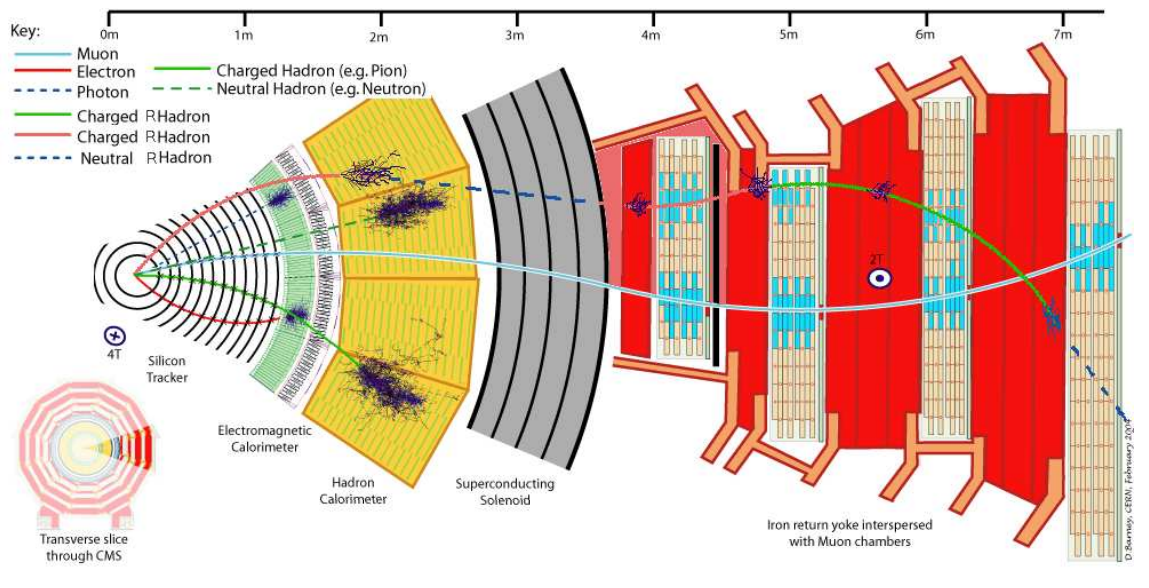
\includegraphics[width=\plotwidth]{fig/chapt3/CMS-slice-HSCPs.png}
		\caption{\label{fig:HSCPs} Slice of the CMS detector showing example of passage of SM particles and R-hadrons. On the one hand, lepton-like HSCPs will appear to behave like slow and heavy muons. On the other hand, R-hadrons are likely to convert into other kind of charged or neutral R-hadrons due to interactions inside the detector volume.}
	\end{figure}
	
\section{Desciption of the muon system}
\label{chapt3:sec:muonsystem}
	
	The barrel region is divided into 5 \textit{wheels} made out of 4 \textit{rings} of detectors with iron return yokes in between them whereas the endcaps are made out of 4 disks, each divided into pseudorapidity stations, 2 for CSCs (except for the first disk where 3 stations are equipped) and 3 for RPCs, although only 2 RPCs stations are equipped at present. The wheels and disks are shown in Figure~\ref{fig:Muon}. So far, each subsystem was dedicated to a particular task. DTs, in the barrel, and CSCs, in the endcaps, are used mainly for their spatial resolution. Indeed, DTs' resolution is of the order of \SI{100}{\micro m} along both the $(r-\phi)$ and $(r-z)$ components while the resolution of CSCs is similar but varies in a range from \SI{50}{\micro m} to \SI{140}{\micro m} depending on the distance to the beamline. On the other hand, RPCs are used for their time resolution as they can deliver an information on the muon tracks within \SI{1.5}{ns}.
	
	\begin{figure}[H]
		\begin{subfigure}{0.35\linewidth}
			\centering
			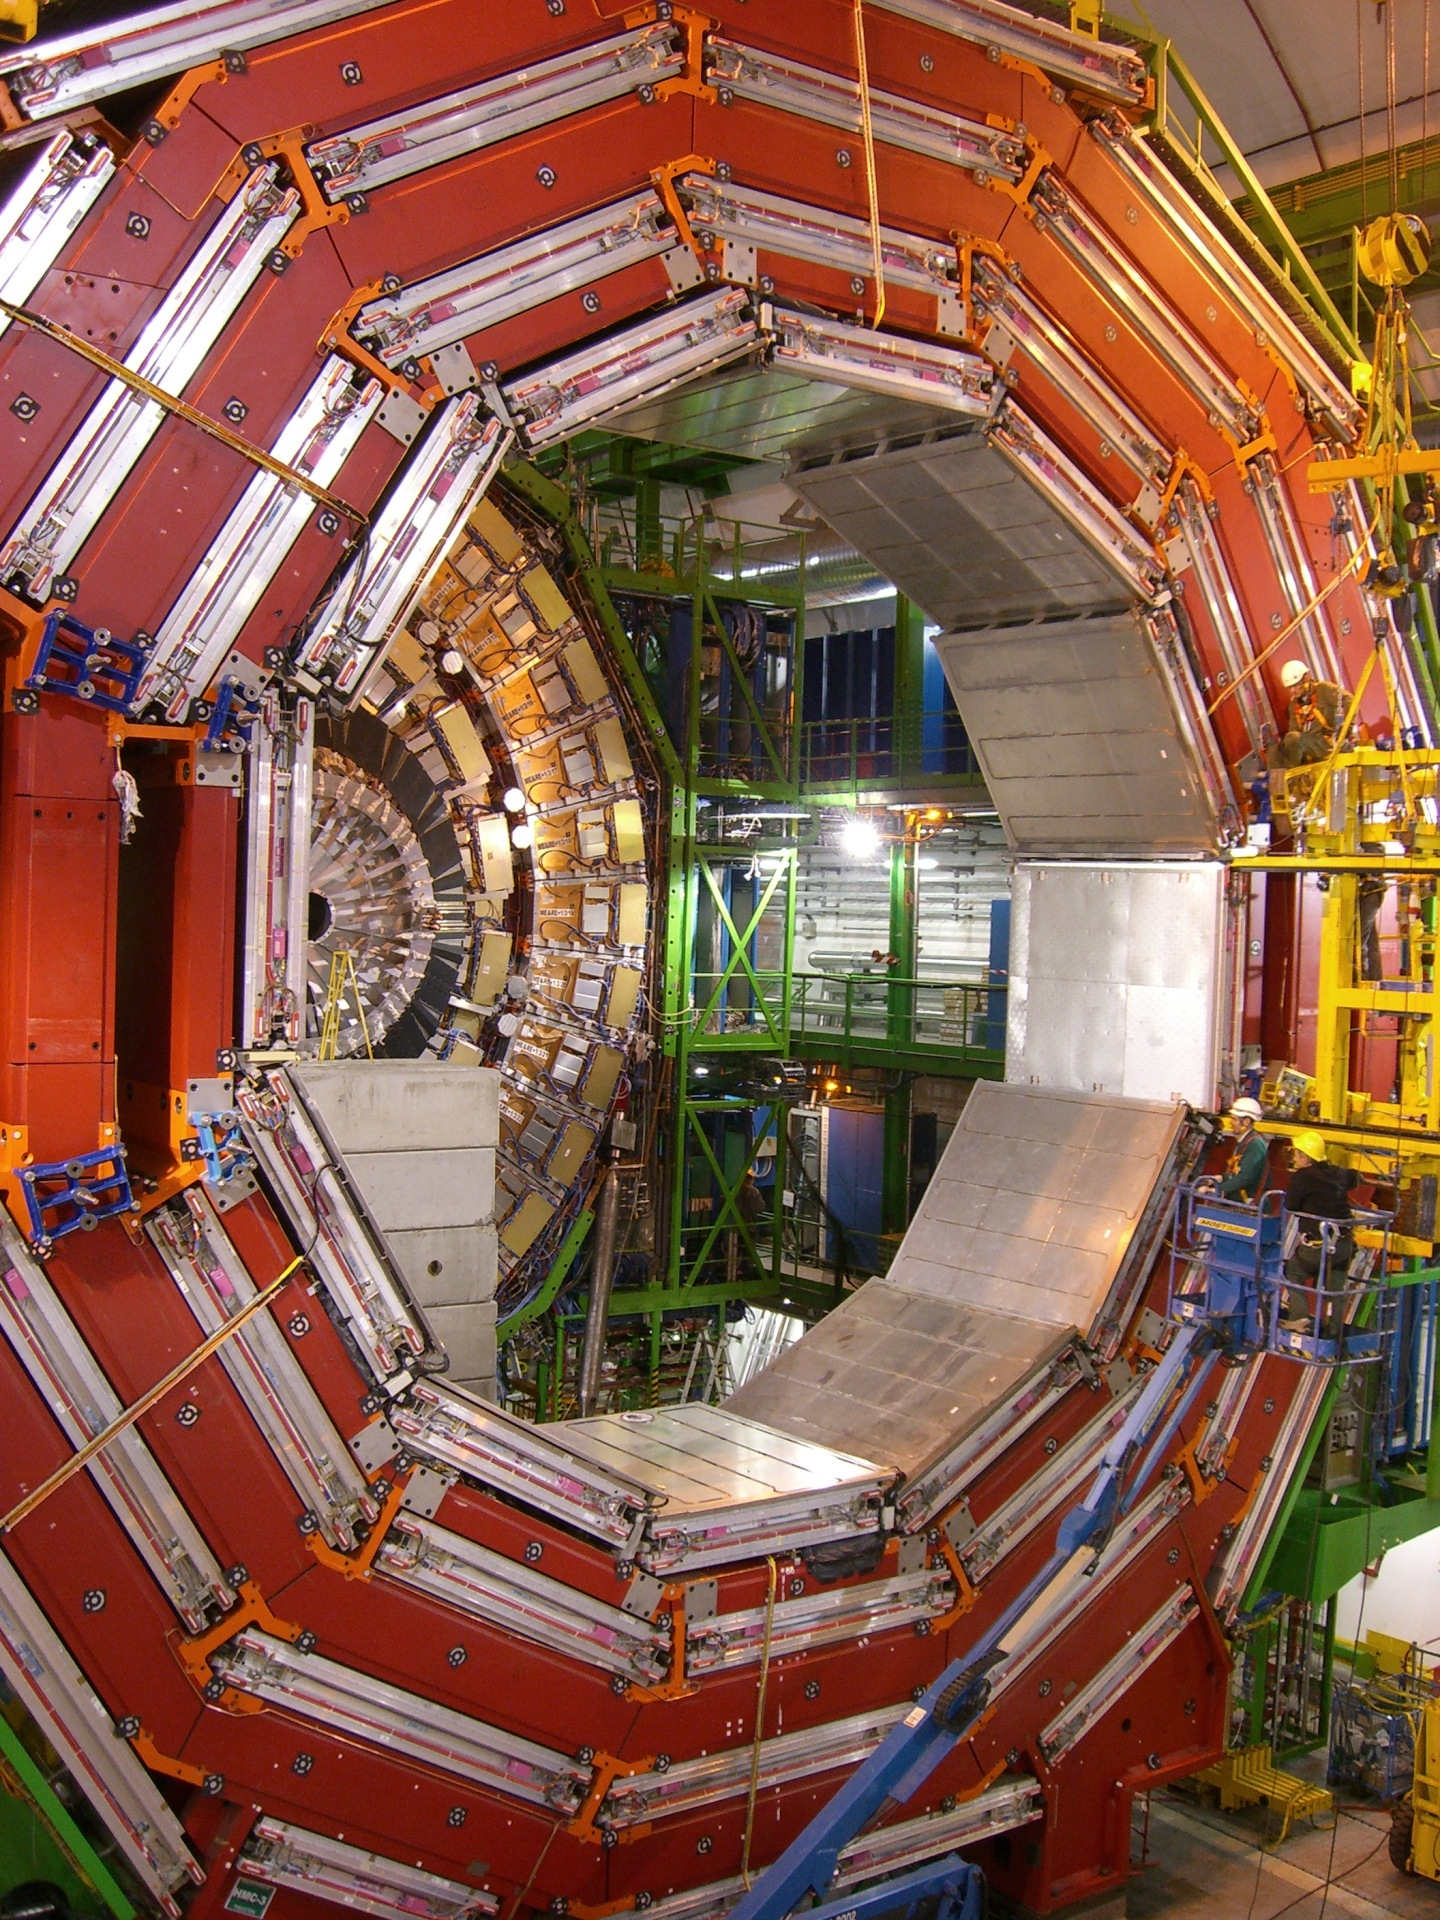
\includegraphics[height = 6cm]{fig/chapt2/Wheel.jpg}
			\caption{\label{fig:Muon:A}}
		\end{subfigure}
		\begin{subfigure}{0.3\linewidth}
			\centering
			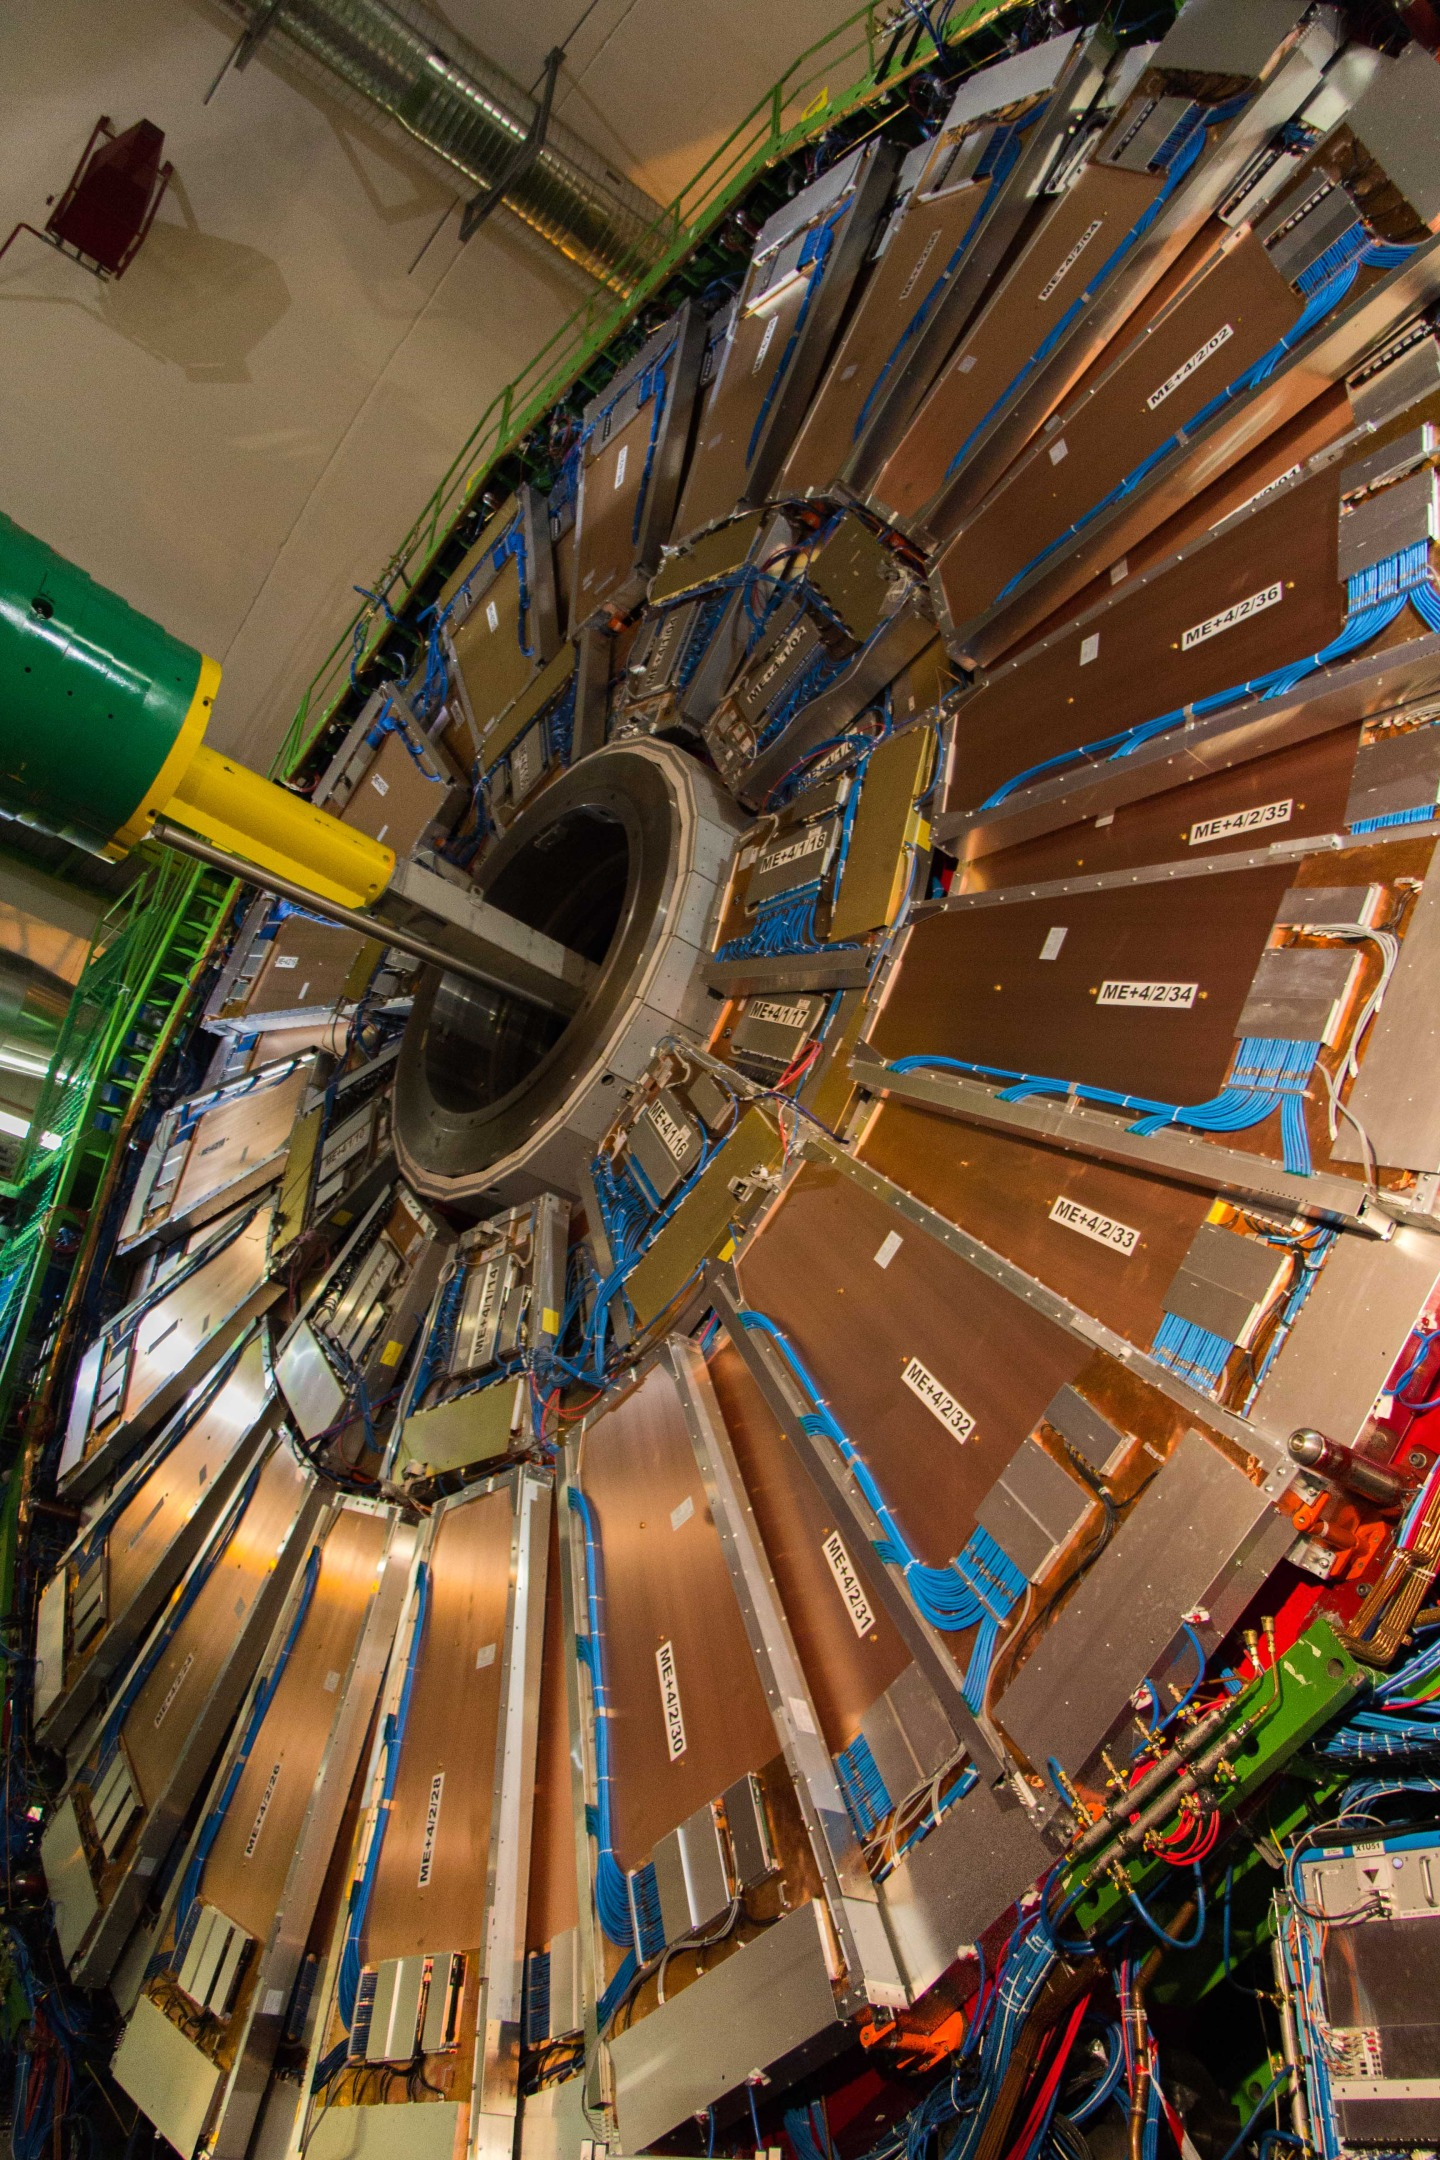
\includegraphics[height = 6cm]{fig/chapt2/Disk_CSC.jpg}
			\caption{\label{fig:Muon:B}}
		\end{subfigure}
		\begin{subfigure}{0.35\linewidth}
			\centering
			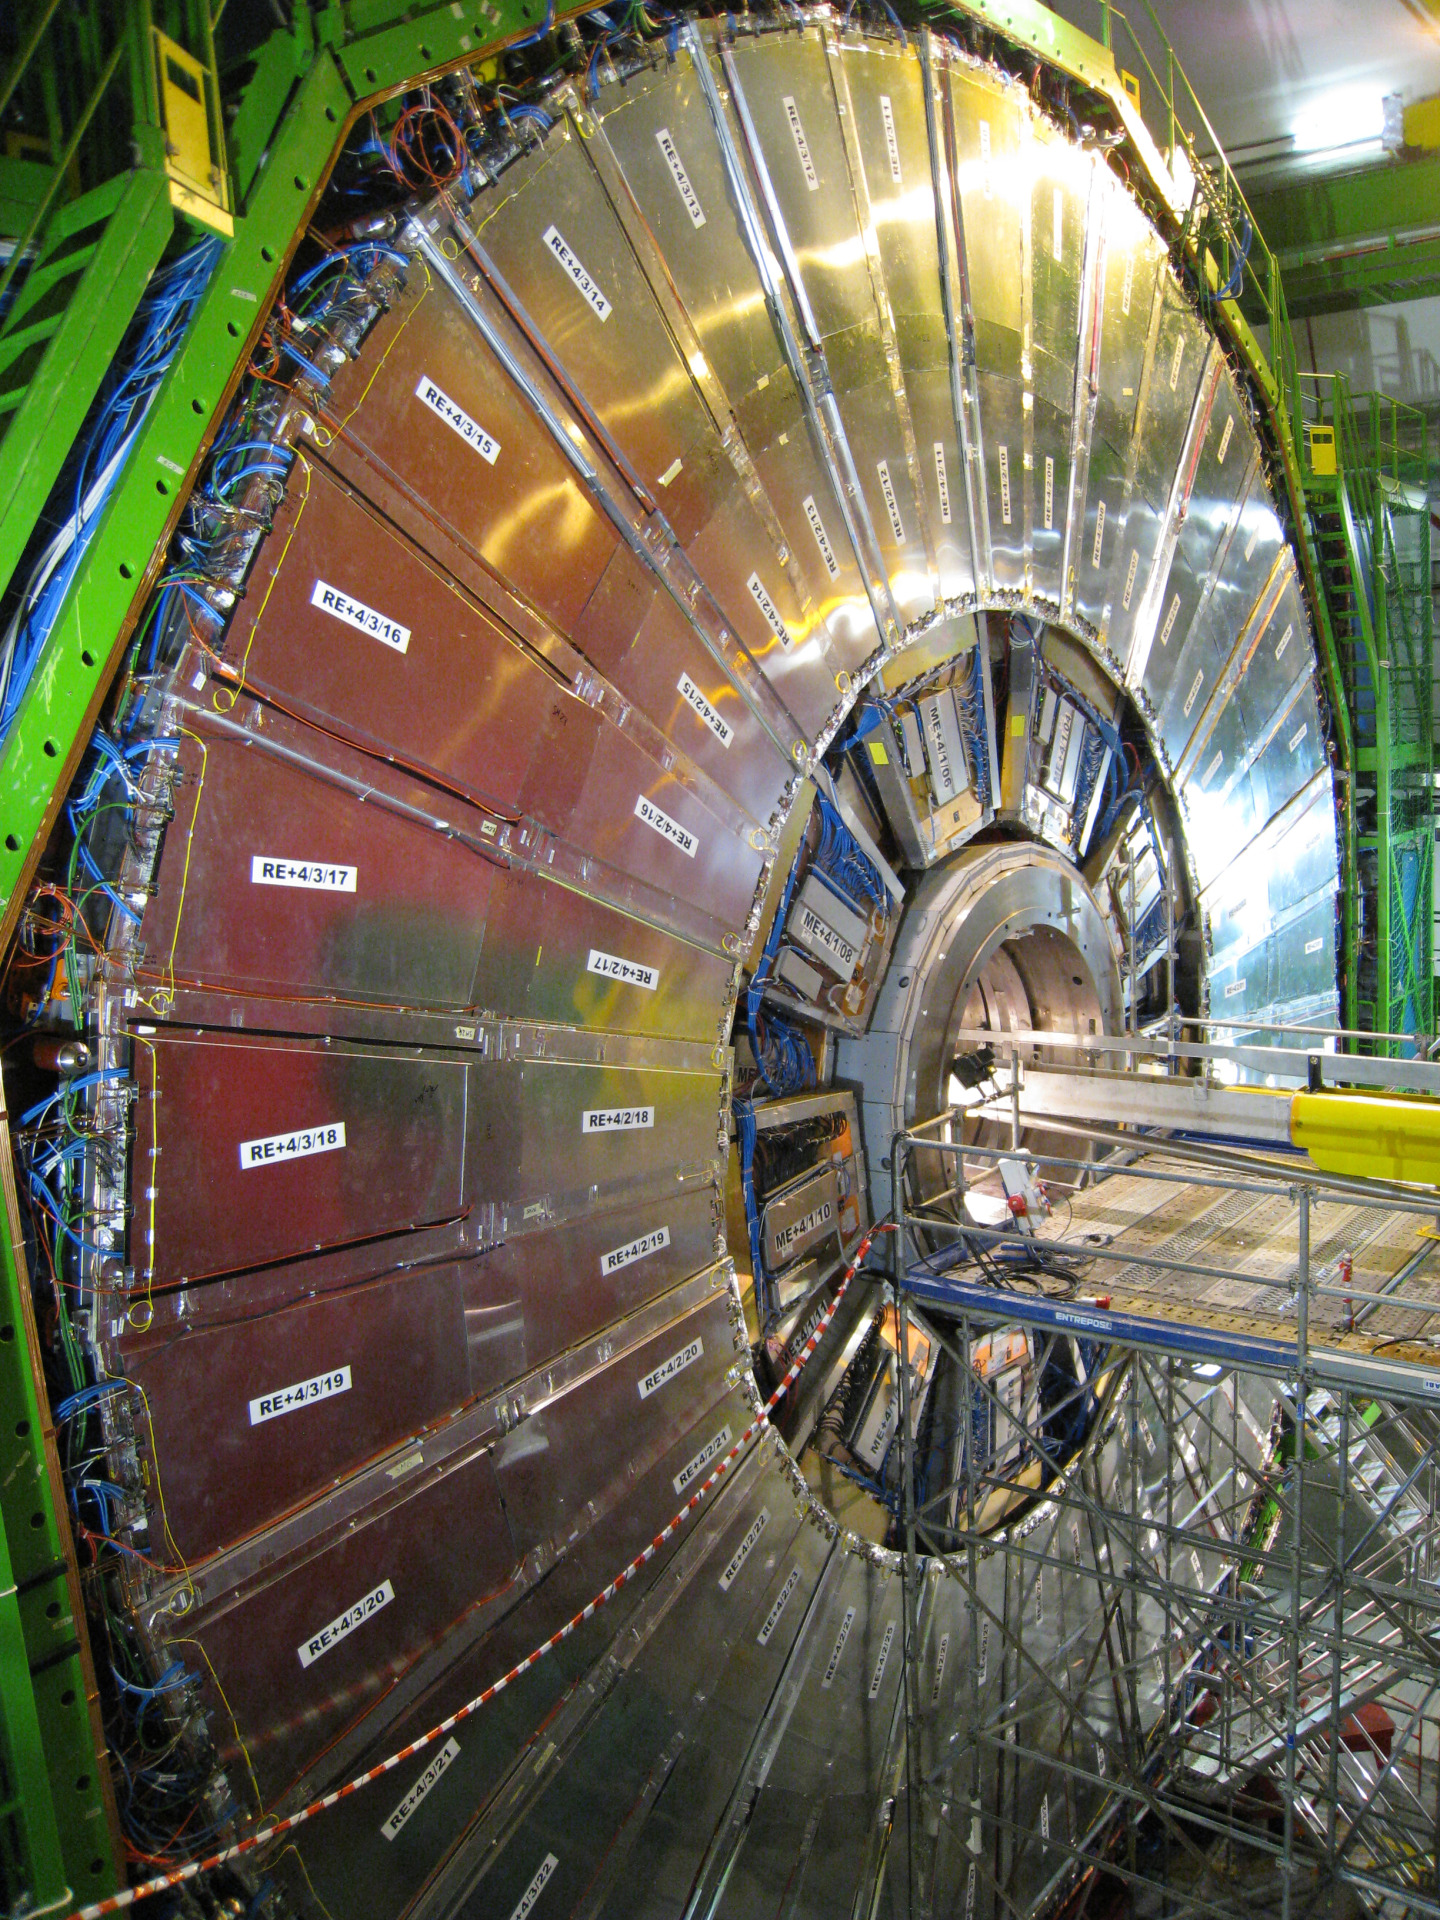
\includegraphics[height = 6cm]{fig/chapt2/Disk_RPC.jpg}
			\caption{\label{fig:Muon:C}}
		\end{subfigure}
		\caption{\label{fig:Muon} Figure~\ref{fig:Muon:A}: Barrel wheel with its detector rings and return yokes. Figure~\ref{fig:Muon:B}: CSC endcap disk with the 2 CSC stations. The outer station is made of \SI{10}{\deg} detectors while the inner station is made of \SI{20}{\deg} detectors. Figure~\ref{fig:Muon:C}: RPC endcap disk. The inner station is not equipped and the inner CSC station can be seen.}
	\end{figure}
	
	\begin{figure}[H]
		\begin{subfigure}{0.6\linewidth}
			\centering
			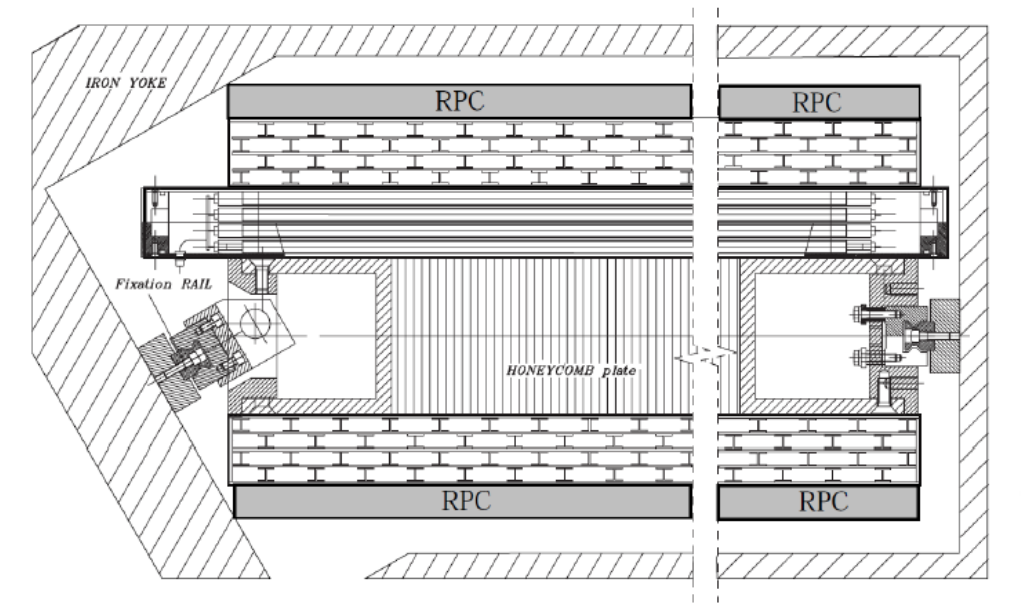
\includegraphics[height = 4.5cm]{fig/chapt2/DT_layout.png}
			\caption{\label{fig:DT:A}}
		\end{subfigure}
		\begin{subfigure}{0.4\linewidth}
			\centering
			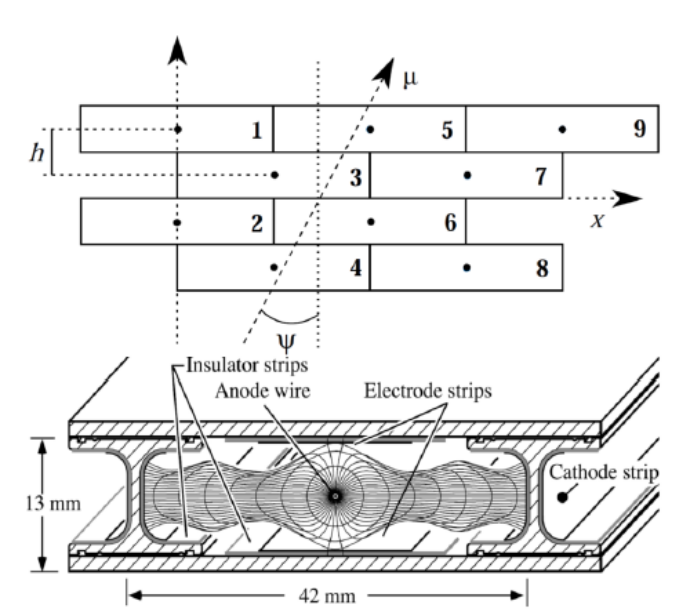
\includegraphics[height = 4.5cm]{fig/chapt2/DT_cells.png}
			\caption{\label{fig:DT:B}}
		\end{subfigure}
		\caption{\label{fig:DT} Figure~\ref{fig:DT:A}: Cross section of a DT module showing the two superlayers measuring the $\phi$ coordinate, perpendicular to the cross section plane, and the superlayer measuring the $\eta$ coordinate, placed in between the two others with honeycomb and parallel to the cross section plane. The DT detector is sandwiched in between 2 RPCs whose readout strips are perpendicular to the cross section plane, measuring the $\phi$ coordinate. Figure~\ref{fig:DT:B}: A DT cell is shown together with its electric field. The path of a muon through a superlayer is shown.}
	\end{figure}
	
	The 250 CMS DTs, found in the barrel covering the pseudorapidity region \psrapr{0}{1.2} and whose structure is shown in Figure~\ref{fig:DT}, are composed of 3 \textit{superlayers} of DT cells. Two of these superlayers are dedicated to measuring the $\phi$ coordinate of the muons and while the last one measures the $\eta$ (or $z$) coordinate. Each superlayer consists on 4 layers of 60 to 70 DT cells arranged in quincunx to allow for a precise reconstruction of the muon path through the DT layers. Each DT cell is a rectangular aluminium gas volume with a central anode wire. Cathode strips are placed on the narrow surface of the cells and electrode strips are placed on the wide surface to help shaping the electric field to ensure a consistent drift velocity of electrons in the drift volume. These detectors are operated using a 85/15 mixture of $Ar$ and $CO_2$.
	
	\begin{figure}[H]
		\begin{subfigure}{0.4\linewidth}
			\centering
			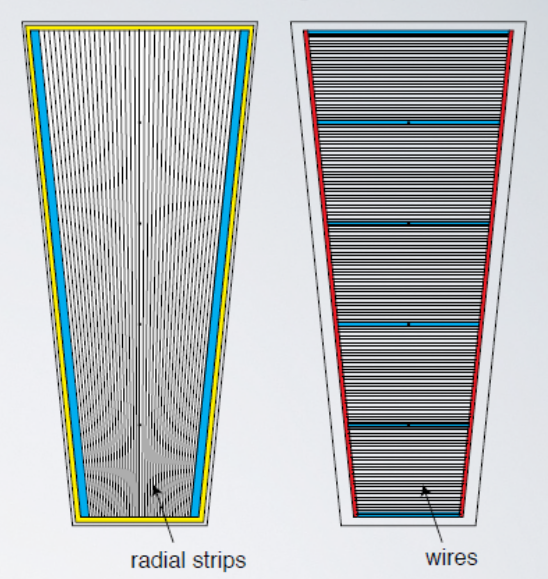
\includegraphics[height = 5cm]{fig/chapt2/CSC_layout.png}
			\caption{\label{fig:CSC-layout:A}}
		\end{subfigure}
		\begin{subfigure}{0.6\linewidth}
			\centering
			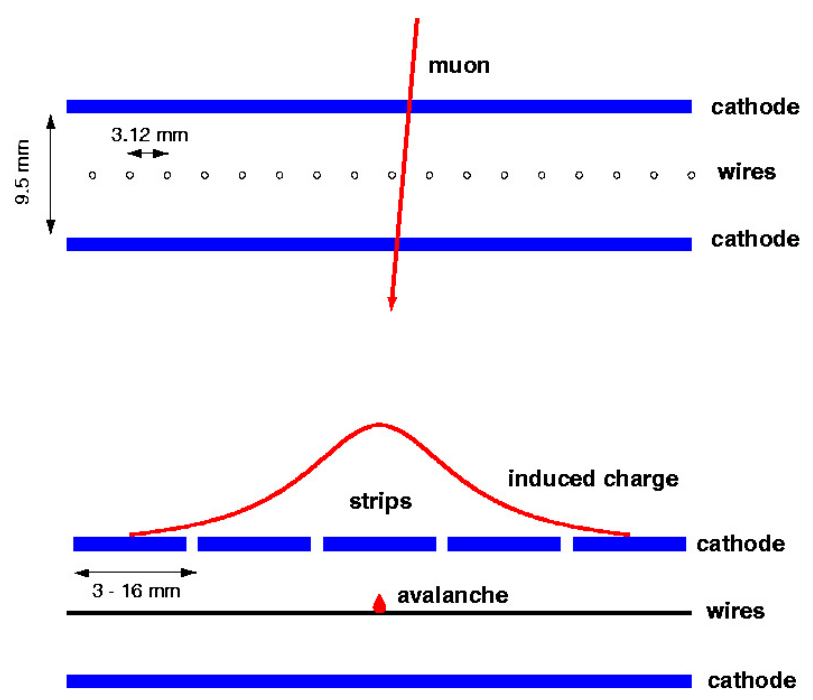
\includegraphics[height = 5cm]{fig/chapt2/CSC_avalanche.png}
			\caption{\label{fig:CSC-layout:B}}
		\end{subfigure}
		\caption{\label{fig:CSC-layout} Figure~\ref{fig:CSC-layout:A}: cathode strips and anode wire layout of a CSC panel. Figure~\ref{fig:CSC-layout:B} avalanche development and charge collection by anode wires and induction on cathode strips inside of a CSC panel.}
	\end{figure}
	
	\begin{figure}[H]
		\centering
		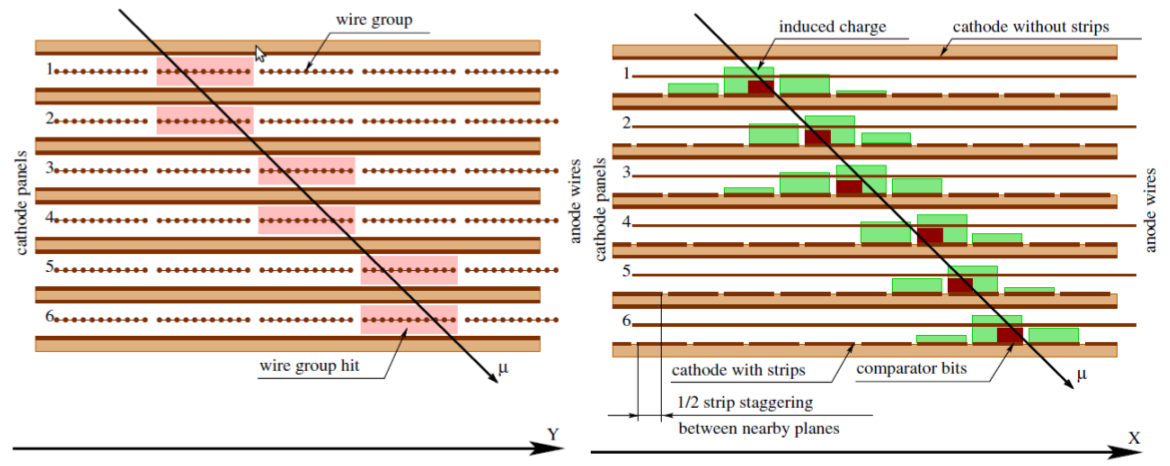
\includegraphics[width=\textwidth]{fig/chapt2/CSC_track.png}
		\caption{\label{fig:CSC-track} Muon track reconstruction through the 6 panels of a CMS CSC using the information of anode wire groups and cathode strip charge distribution combined with comparator bits to decide on which half strip the muon is more likely to have passed.}
	\end{figure}
	
	The 540 CMS CSCs, found in the endcaps covering the pseudorapidity region \psrapr{0.9}{2.5} and described through Figures~\ref{fig:CSC-layout} and \ref{fig:CSC-track}, are composed of 6 panels of CSC, each panel consisting in a wide gas volume of \SI{9.5}{mm} (\SI{7}{mm} in the case of ME1/1 station) containing anode wires and whose surfaces are cathodes. The top cathode is a wide copper plane of the size of the gas volume. The bottom cathode is divided into thin trapezoidal copper strips radially arranged to measure the azimuthal coordinate $\phi$ with a pitch ranging from 8 to \SI{16}{mm}. The \SI{0.50}{\micro m} anode wires are placed perpendicularly to the strips to measure radial coordinate $r$ and are grouped by 10 to 15 with a wire to wire space of \SI{3.2}{mm}. In he specific case of ME1/1 placed against the HCAL endcap, the \SI{0.30}{\micro m} anode wires have a wire to wire distance of \SI{2.5}{mm} and are not disposed perpendicularly to the strips but slightly tilted by an angle of \SI{29}{\deg} to compensate for the lorentz force due to the very strong local magnetic field of \SI{4}{T}. These detectors are operated with a 40/50/10 mixture of $Ar$, $CO_2$ and $CF_4$. Combining the information of the multiple CSC panels, the detectors achieve a very precise measurement of the muon track.
	
	Despite their excellent spatial resolution, the wire chambers (DTs and CSCs) are limited in terms of time resolution by the fact that the charge needs to drift towards the anode wire and be collected before having the confirmation that a particle was detected as the drift volume is not used to develop avalanches. Indeed, the stronger electric field close to the anode wire triggers the avalanche and the gain of the detector. Due to the drift, the time resolution is thus limited at best to approximately 2 to \SI{3}{ns}. In addition, even though the intrinsic time resolution of the tracking chambers is rather good compared to the \SI{25}{ns} in between successive collisions, the processing time of the trigger system doesn't allow for very fast triggering as it provides a time precision of only \SI{12.5}{ns}. Thus, detectors fully dedicated to timing measurement have been installed as a redundant system. These detectors are RPCs, also gaseous detectors but that use current induction instead of charge collection allowing for a time resolution of the order of \SI{1.5}{ns} only. Theoretically, depending on the design used, RPCs could reach a time resolution of the order of \SI{10}{ps} but in the context of LHC where bunch crossing happen every \SI{25}{ns}, a time resolution of \SI{1.5}{ns} is sufficient to accurately assign the right bunch crossing to each detected muon.
	
	The 1056 RPCs equipping the CMS muon system both in the barrel and endcap regions and covering the pseudorapidity region \psrapr{0}{1.6} are composed of two layers of RPC \textit{gaps} as described in Figure~\ref{fig:RPC-DG-layout}. Each gap consists in two resistive electrodes made out of \SI{2}{mm} thick Bakelite enclosing a \SI{2}{mm} thick gas volume containing a 95.2/4.5/0.3 mixture of $C_2H_2F_4$, $i-C_4H10$ and $SF_6$. Due to this geometry, the electric field inside of a gap is homogeneous and linear at every point in the gas translating into a uniform development of avalanches in the gas volume as soon as a passing muon ionises the gas. The two gaps sandwich a readout copper strip plane. A negative voltage is applied on the outer electrodes, used as cathodes, and the inner electrodes, the anodes, are simply connected to the ground as well as the readout panel that picks up the current induced by the accumulated charge of the growing avalanches in one or both of the gas gaps. This OR system allows for a lower gain (i.e. a lower electric field) on both gaps to reach the maximal efficiency of such a detector.
	
	\begin{figure}[H]
		\centering
		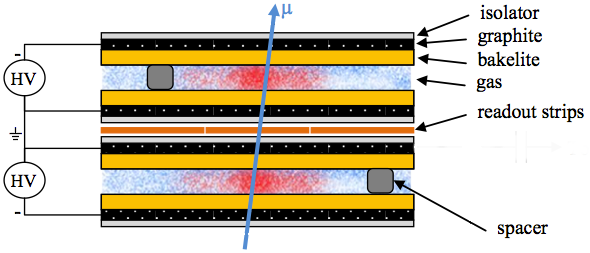
\includegraphics[width=0.7\textwidth]{fig/chapt2/RPC_DG_layout.png}
		\caption{\label{fig:RPC-DG-layout} Double gap layout of CMS RPCs. Muons passing through the gas volumes will create electron-ions pairs by ionising the gas. this ionisation will immediately translate into a developing avalanche.}
	\end{figure}
	
\section{Muon system requirements for HL-LHC}
\label{chapt3:sec:requirements}

	The increase of irradiation close to the beam line will affect the background rate seen by the muon detectors in this area and tracking muons will prove to be difficult as this region is not yet equipped with all the detectors that were already foreseen for Phase-I. Improving this situation will come with the increase of hit numbers recorded along the particle track to reduce the ambiguity on muon versus background detection. Moreover, the measurement of small production cross-section and/or decay branching ratio processes, such as the Higgs boson coupling to charge leptons, and in particular to muons, or the $B_s \longrightarrow \mu^+\mu^-$ decay, is of major interest and specific upgrades in the forward regions of the detector will be required to maximize the physics acceptance to the largest possible solid angle.

	\begin{figure}[H]
		\centering
		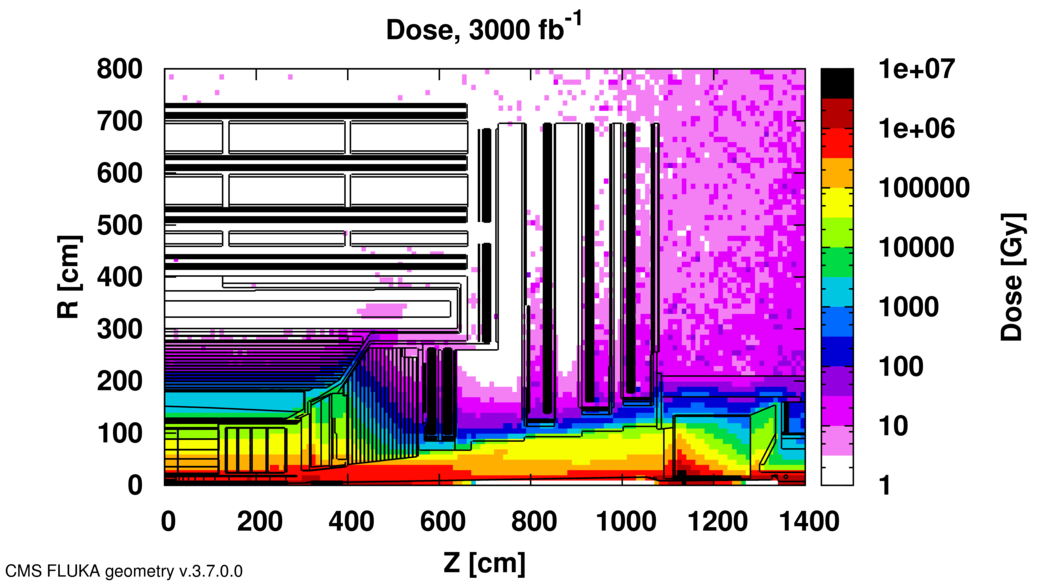
\includegraphics[width=0.7\textwidth]{fig/chapt3/HL-LHC-Dose.png}
		\caption{\label{fig:Dose} Absorbed dose in the CMS cavern after an integrated luminosity of \SI{3000}{\femto\per\barn}. Using the interaction point as reference, R is the transverse distance from the beamline and Z is the distance along the beamline.}
	\end{figure}
	
	\begin{figure}[H]
		\centering
		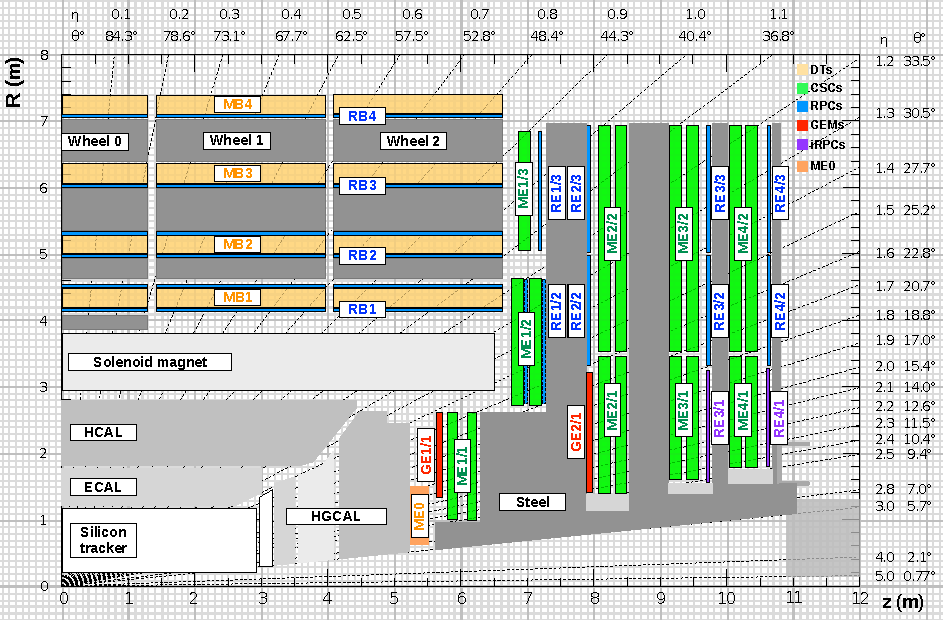
\includegraphics[width=0.7\textwidth]{fig/chapt3/Phase2_Muon_quadrant.pdf}
		\caption{\label{fig:P2Quadrant} A quadrant of the muon system, showing DTs (yellow), RPCs (blue), and CSCs (green). The locations of new forward muon detectors for Phase-II are contained within the dashed box and indicated in red for GEM stations (ME0, GE1/1, and GE2/1) and dark blue for improved RPC (iRPC) stations (RE3/1 and RE4/1).}
	\end{figure}
	
To ensure proper trigger performance within the present coverage, the muon system will be completed with new chambers and the electronics of the present system will need to be upgraded to ensure an efficient triggering. Figure~\ref{fig:P2Quadrant} shows the addition of \acf{GEM} and \acf{iRPC} in the pseudo-rapidity region $1.6<\vert\eta\vert<2.4$ to complete the redundancy of the already existing CSCs as originally scheduled in the CMS Technical Proposal~\cite{CMSTP}. A first step into this direction will be taken by installing GEMs on the first endcap disk in position GE1/1 during LS2, during which preparations for the future installation of more GEMs and RPCs will take place by installing the needed services. During the YETS following LS2, iRPCs will be installed on the third and fourth endcap disks in position RE3/1 and RE4/1, and more GEMs will equip the second endcap in position GE2/1 and the inner layer, closest to the HCAL endcap called ME0 during LS3, finally completing the redundant coverage of the muon system and extending it a little by extending the reach to \psrape{2.8}, the redundancy in the region \psrapr{2.4}{2.8} being maintained by the 6 GEM layers contained in each ME0 detector that provide enough tracking points to efficiently reject neutron-induced background.
	
	Nevertheless, the region beyond \psrapg{2.8} and extending to \psrape{5.0} only is covered by the forward HCAL detectors and lack redundant muon detector coverage. Extensions of the tracker in the context of HL-LHC will increase its coverage up to \psrape{4.0} but the identification of muons and measurement of their energy with reasonable precision only using the tracker is nearly impossible. Thus, this increased tracker coverage range needs to be put in parallel with a matching muon detector and will open doors to multi-lepton final states in which leptons are likely to have a a low transverse momentum and to be found near the beam line.
	
	Finally, as the muon system is composed only of gaseous detectors, strong environmental concerns have risen over the last years as the European directives will restrict the use of fluorine based gas mixtures. Both the CSC and RPC subsystems, using $CF_4$, $C_2H_2F_4$, or $SF_6$, will need to adapt their working gas in order to strongly reduce the greenhouse potential of the mixtures released into the atmosphere due to gas leaks.
	
\section{Necessity for improved electronics}
\label{chapt3:sec:electronics}

	Drift Tubes and Cathode Strip Chambers are important components used to identify and measure muons, especially thanks to their spatial resolution of the order of \SI{100}{\micro m}. Nevertheless, the luminosity and irradiation during HL-LHC will cause serious event loss and ageing on the electronics of these subsystems that will comprise the triggering and data transfering needs of CMS. Thus, electronics upgrade are foreseen to address these expected problems. While only the RPCs' electronic system is able to operate under Phase-II requirements, DTs and CSCs will need to improve their trigger accept rate and latency to ensure that Level-1 trigger threshold stays at the same level~\cite{LEVEL1IR}, and DAQ data transfer rate, that respectively need to achieve a minimum of \SI{500}{kHz}, get down to \SI{12.5}{\micro s}~\cite{CMSIITP}, and increase to \SI{1082}{Gbit/s} DTs and to \SI{1026}{Gbit/s} for CSCs. As of today, the Level-1 trigger accept rate of DTs doesn't reach \SI{300}{kHz} while this of CSCs is bellow \SI{250}{kHz} but the foreseen upgrades are expected to increase the rate way beyond the requirement in the of DTs and up to \SI{4}{MHz} for CSCs~\cite{PHASEIITP}.
	
	The \acf{MiC1} used by DTs don't allow for high enough trigger rate. In addition to this problem, it was showed that these electronics contain components that are not radiation hard enough to sustain HL-LHC conditions and thus, a too large number of channels may fail due to radiations. The MiC1 will be replaced on each detector by an improved version referred to as MiC2 while front-end electronics and high-voltage modules will not need any replacement. On the other hand, CSCs showed that there electronics would be able to live through the 10 years of Phase-II but the limited buffer depth might cause memory overflows and readout inefficiencies with a fraction of event loss ranging from 5 to more than 10\% at an instantaneous luminosity similar to which of HL-LHC depending on the expected background. Thus the replacement of CSCs' \acf{CFEBs} by digital ones, DCFEBs, with deeper buffer would permit to make event loss negligible and satisfy HL-LHC requirements~\cite{PHASEIITP}. All these new DT and CSC electronics will be connected to the trigger electronics via optical links to ensure a faster communication.
	
	\begin{figure}[H]
		\centering
		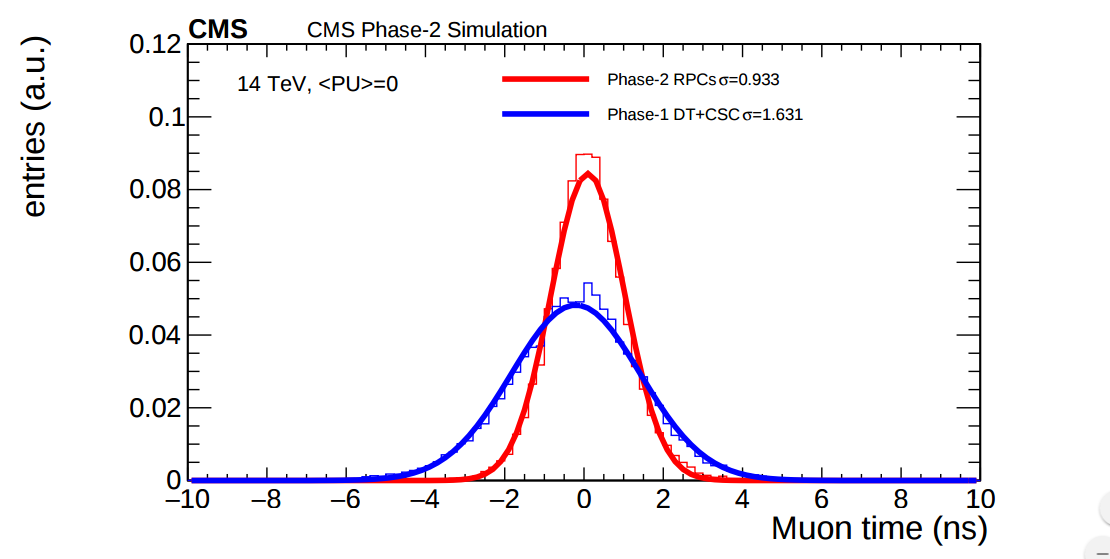
\includegraphics[width=\plotwidth]{fig/chapt3/RPC-ugrade-LS.png}
		\caption{\label{fig:RPC-time} Comparison of the simulated time residuals in between reconstructed and true muon times without (blue) and with (red) the upgraded RPC link system.}
	\end{figure}
	
	The upgrade on the side of Resistive Plate Chambers will then not come from their on-board electronics but from the Link System located in the service cavern of CMS and that connects the front-end electronics data of RPCs into CMS trigger processors. The main motivation for such and upgrade is that the electronic board composing the link system are built using obsolete components and weak components that can easily suffer from the electromagnetic noise. These components may be the source of failing channels throughout Phase-II. Moreover, these link boards were originally designed only to match RPC digitized signals with the corresponding bunch crossing. Due to this feature, the time resolution of the full RPC chain is thus limited to \SI{25}{ns} and does not exploit the full time resolution of the detectors. This would make the synchronization of the RPC system easier and allow to have a finer offline background removal within the \SI{25}{ns} in between bunch crossings thanks to the order of magnitude gained in terms of time resolution.
	
	Upgrading RPC link system will require the installation of 1376 new link boards and 216 control boards. The new boards will make use of the recent progress made with fast FPGAs and will be a great improvement to the ASICs formerly used as they will be able to process signals from several detectors in parallel. The benefice from using the full RPC time resolution thanks to the upgraded link system can be seen through Figure~\ref{fig:RPC-time} where the resolution of the RPC system itself is better than which of DTs and CSCs that was used until now.

\section{New detectors and increased acceptance}
\label{chapt3:sec:GEMRPC}

	In the present muon system, the redundancy of was assured by RPCs used for their good timing performances. The extension of the muon system towards higher pseudo-rapidity in order to complete the redundancy in this very region and to contribute to the precision of muon momentum measurements will require muon chambers with a spatial resolution less or comparable to the contribution  muon of multiple scattering through the detector volume~\cite{MUONTDR}. Most of the plausible physics is covered only considering muons with $p_T<$\SI{100}{GeV} hence, in order to match CMS requirements, a spatial resolution of $\mathcal{O}$(few $\mathrm{mm}$) will be necessary for the proposed new RPC stations while the GEMs will need a resolution better than \SI{1}{mm}, as showed by the simulation in Figure~\ref{fig:MultiScat}.

	\begin{figure}[H]
		\centering
		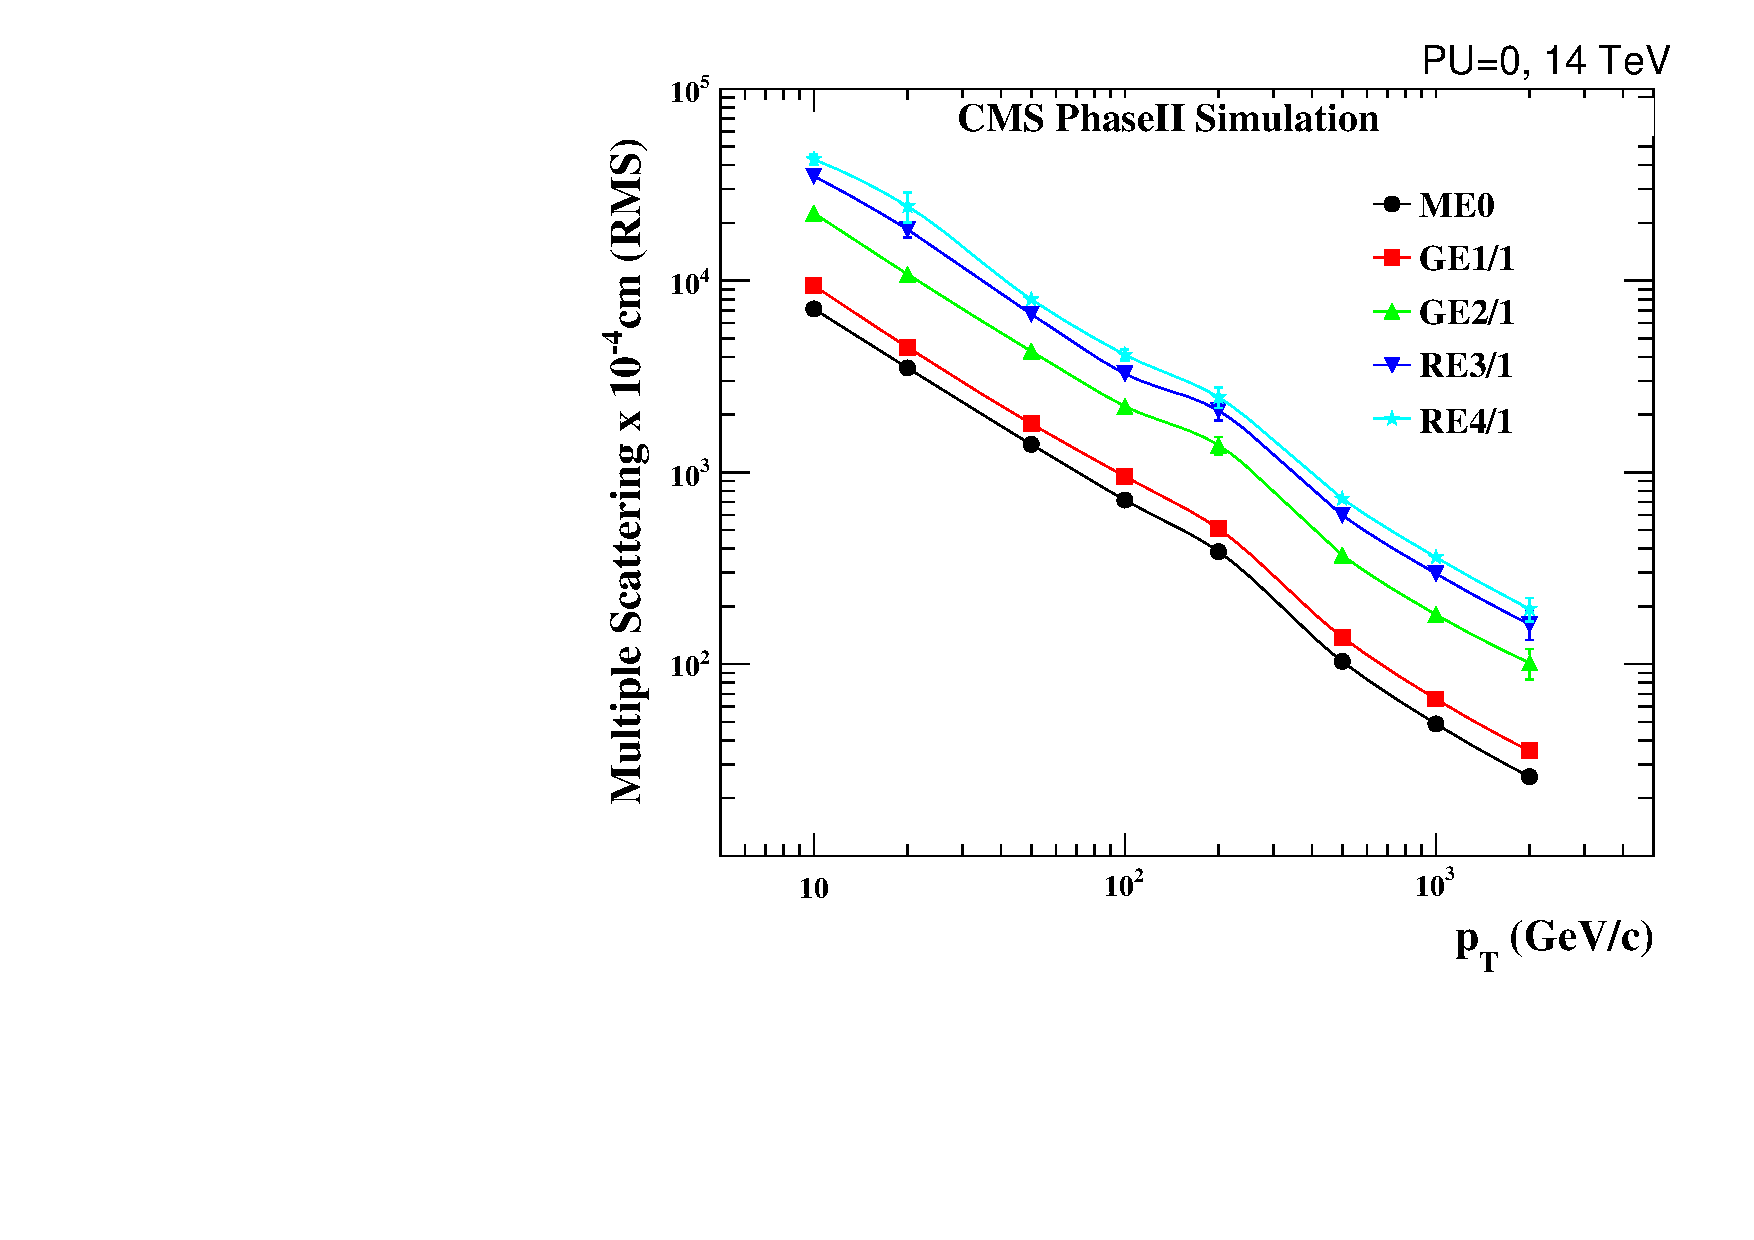
\includegraphics[width=0.6\textwidth]{fig/chapt3/MS_allstations.pdf}
		\caption{\label{fig:MultiScat} RMS of the multiple scattering displacement as a function of muon $p_T$ for the proposed forward muon stations. All of the electromagnetic processes such as bremsstrahlung and magnetic field effect are included in the simulation.}
	\end{figure}
	
	\subsection{Gas electron multipliers}
	\label{chapt3:ssec:GEMs}
	
	In the region closer to the interaction point where the spatial resolution is requested to be better than \SI{1}{mm} for the new detectors (at least for GE1/1 and ME0, GE2/1 being in the same order of requested spatial resolution than the new iRPCs that will equip the third and fourth endcaps), the choice has been made to use triple GEMs, micro pattern gaseous detectors, in the place of RPCs. The GE1/1 project had been the first to be approved and demonstrators had been installed in CMS already during LS1. The rest of the detectors will be installed during LS2 while the GE2/1 and ME0 projects are still under development. ME0, GE1/1 and GE2/1 will be installed respectively next to the HCAL endcap, on the first and on the second muon endcap disks as can be seen from Figure~\ref{fig:P2Quadrant}.

	\begin{figure}[H]
		\centering
		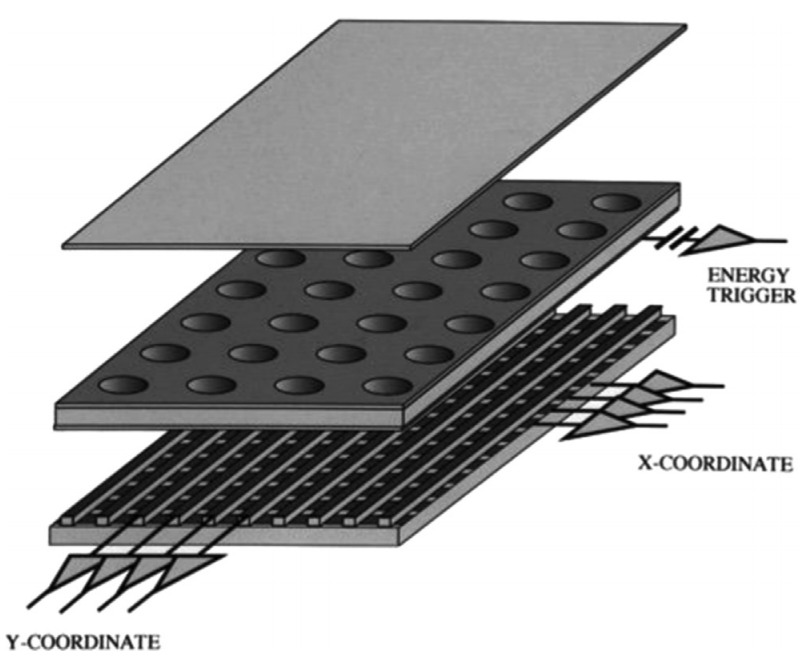
\includegraphics[width=0.5\plotwidth]{fig/chapt3/GEM.png}
		\caption{\label{fig:GEM} Schematics of a GEM showing the cathode on top, the GEM foil separating the gas volume into the drift region, in between the cathode and foil, and the induction region, in between the GEM foil and the anode, and the anode on which a 2D read-out is installed. A negative voltage is applied on the cathode while the anode is connected to the ground.}
	\end{figure}
	
	Gas Electron multipliers are gaseous detectors~\cite{SAULI97} which gas volume is confined in between 2 planar electrodes, the anode serving as read-out panel. The gas volume is divided in 2 or more regions by a single or multiple \textit{GEM foils} as showed in Figure~\ref{fig:GEM}. These foils are very thin, of the order of a few tens of \si{\micro m}, and are pierced with holes as can be seen in Figure~\ref{fig:GEM-foil}. Both surfaces of the GEM foils are clad with copper in order to apply a strong electric field in between each side that will generate very strong potentials in the holes. The gas region contained in between the cathode and the GEM foil is called the drift region as the electric field is not strong enough to cause avalanches and thus start an amplification. The primary electrons drift toward the foil and are accelerated and amplify by the very high potential within the holes, as showed in Figure~\ref{fig:GEM-foil}. Then the electrons reach the second drift region in which they will induce signal on the read-out located on the anode. By restraining the amplification process at the level of the holes, the electrons can stay in a very confined space and thus induce a very localized current, providing the GEMs with a very good spatial resolution.

	\begin{figure}[H]
		\centering
		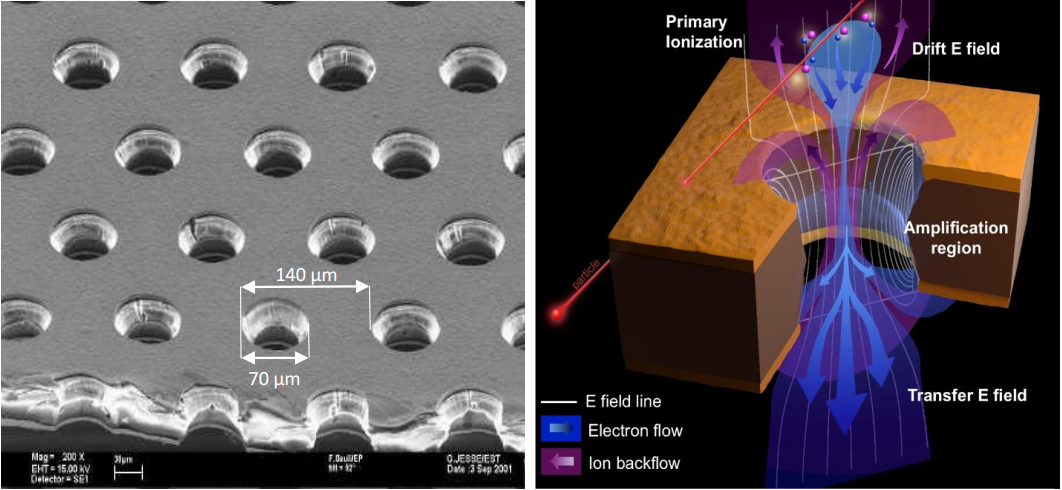
\includegraphics[width=\plotwidth]{fig/chapt3/GEM-foil-ampli.png}
		\caption{\label{fig:GEM-foil} Left: Picture of a CMS GEM foil provided by a scanning electron microscope. Righ: Representation of the electric field lines in a GEM hole and of the amplification that electrons and ions undergo in the hole's volume due to the very intense electric field.}
	\end{figure}

	\begin{figure}[H]
		\centering
		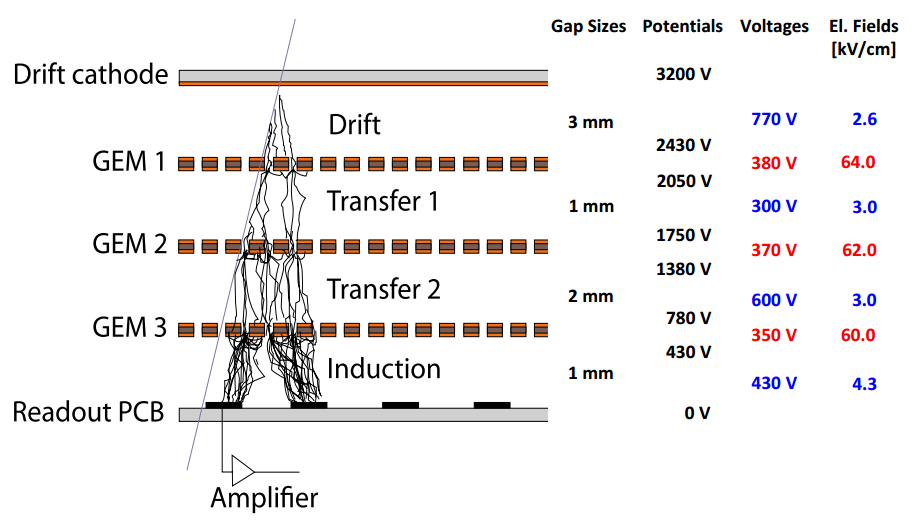
\includegraphics[width=0.8\plotwidth]{fig/chapt3/GEM-drift.png}
		\caption{\label{fig:GEM-drift} Schematic representation of CMS triple GEMs. The gas volume is divided into 4 areas. The drift area is the region where the primary electrons are created before being amplified a first time while passing through the first GEM foil. Then the process of drift and amplification is repeated twice in following two transfer areas and GEM foils. Finally, the charges have been amplified enough to induce current in the read-out strips while in the last drift area. The dimensions, potentials and electric fields are provided.}
	\end{figure}
	
	In order to achieve a stronger amplification, the amplification process can be repeated several times in a row. The GEMs that will be used in CMS are triple GEM detectors operated with a 70/30 gas mixture of $Ar$/$CO_2$. They contain 3 GEM foils and thus 3 electron amplifications, as can be seen in Figure~\ref{fig:GEM-drift}. The GEM foils used in CMS are \SI{50}{\micro m} foils clad with \SI{5}{\micro m} of copper on each side. The foils are pierced with double-canonical holes which inner and outer diameters are respectively 50 and \SI{70}{\micro m} which are placed \SI{140}{\micro m} from each other in an hexagonal pattern, as showed in Figure~\ref{fig:GEM-foil}. These detectors have a time resolution better than \SI{10}{ns} and reach very good spatial resolutions of less than \SI{200}{\micro rad} as indeed the position of the hits is not measured along the strips but following the azimuthal angle granularity of the radialy organized trapezoidal strips.

	\begin{figure}[H]
		\centering
		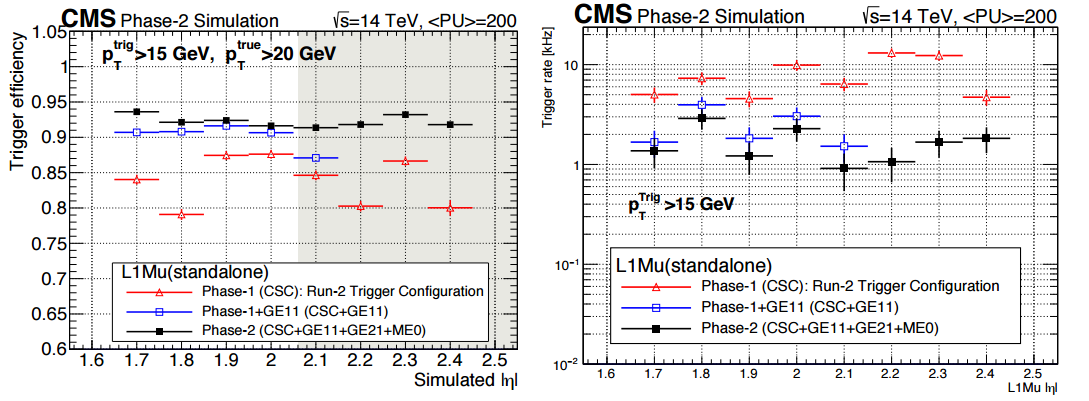
\includegraphics[width=\linewidth]{fig/chapt3/GEM-Trigger.png}
		\caption{\label{fig:GEM-Trigger} Simulated efficiency and rate of the standalone Level-1 muon trigger using tracks reconstructed in CSCs and all GEM stations compared with Phase-I values in the case where only CSCs are used or CSCs+GE1/1. The zones of inefficiency of the CSC subsystem are compensated by the addition of GEMs during Phase-II and the trigger rates is kept from increasing due to the high luminosity.}
	\end{figure}
	
	\begin{figure}[H]
		\begin{subfigure}{0.6\linewidth}
			\centering
			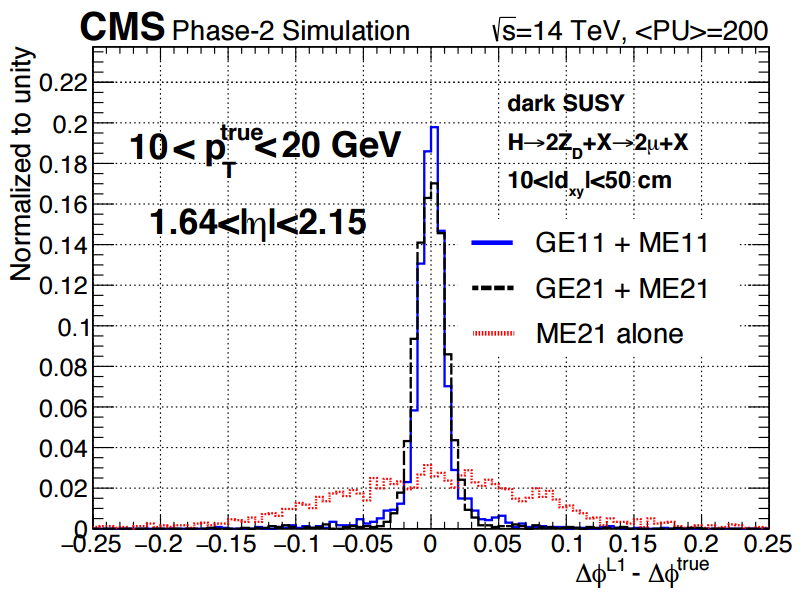
\includegraphics[height=5cm]{fig/chapt3/GEM-muon-direction.png}
			\caption{\label{fig:GEM-Muon:A}}
		\end{subfigure}
		\begin{subfigure}{0.4\linewidth}
			\centering
			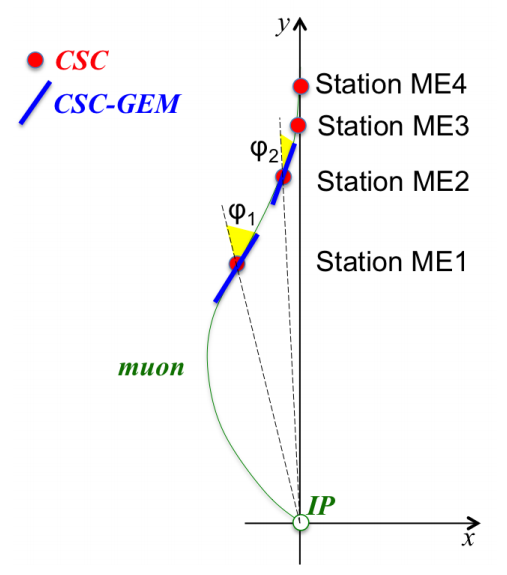
\includegraphics[height=5cm]{fig/chapt3/GEM-Muon-bending.png}
			\caption{\label{fig:GEM-Muon:B}}
		\end{subfigure}
		\caption{\label{fig:GEM-Muon} Figure~\ref{fig:GEM-Muon:A}: Simulated resolution of the muon direction measurement $\Delta\phi$ with Phase-II conditions. In the second endcap station, the resolution is compared in the case of CSCs (ME2/1) alone and CSCs+GEMs (GE2/1+ME2/1) while a similar resolution measurement is given in the case of the first station (GE1/1+ME1/1). Figure~\ref{fig:GEM-Muon:B}: The addition of GEM detectors on stations 1 and 2 (ME0 is considered to contribute to station station 1) as redundant system to CSCs allows to improve the muon momentum improvement through a more accurate measurement of the local bending angles $\phi_1$ and $\phi_2$.}
	\end{figure}
	
	The GEM Upgrade is divided into 3 subsystems as GE1/1 was the first approved project~\cite{GEM11TDR} and that the detectors will already be installed during LS2. GE2/1 and ME0, on the other hand, will profit of the R\&D knowledge and skills developed for GE1/1 while the requirements for each subsystem are different as they are not placed at the same distance from the interaction point. In this very forward region, a different position with respect to the center of the detector can change dramatically the conditions in which the detectors will have to be operated. In terms of rate capability, GE2/1, which is the furthest, is required to withstand \SI{2.1}{kHz/cm^2} while GE1/1 needs to be better than \SI{10}{kHz/cm^2} and ME), better than \SI{150}{kHz/cm^2}. In terms of ageing with respect to charge deposition, ME0 needs to be certified to \SI{840}{mC/cm^2}, GE1/1 to \SI{200}{mC/cm^2} and GE2/1 only to \SI{9}{mC/cm^2}. All 3 detectors need to have a time resolution better than \SI{10}{ns} and an angular resolution better than \SI{500}{\micro rad}.
	
	On each GE1/1 ring, 36 super chambers, consisting of 2 single GEM layers and spanning \SI{10}{\degree}, will be installed covering the pseudo-rapidity region \psrapr{1.6}{2.2} together with ME1/1 CSCs and the reach of the muon system will be improved thanks to the GE2/1 that will overlap with the GE1/1 and cover a region from \psrapg{1.6} to \psrapl{2.4} and complete the redundancy of ME2/1. The super chambers, built with 2 triple GEM layers each consisting of 4 single GEM modules due to the rather large surface of the GE2/1 chambers, that will be installed on the first ring of the second endcap will span \SI{20}{\degree} each, hence, a total of 72 chambers will be assembled to equip the muon system. Finally, the ME0 installed near the HCAl endcap will cover the region \psrapr{2.0}{2.8} and this subsystem will consist in super modules of 6 layers of triple GEM detectors covering an azimuthal angle of \SI{20}{\degree} leading to the construction of 216 single detectors.
	
	Adding the GEMs into the forward region of the muon system will allow to strongly enhance the Level-1 Trigger performance by reducing the inefficiency regions and the trigger rate as showed in Figure~\ref{fig:GEM-Trigger}. Moreover, benefiting from the good spatial and angular resolution of the GEMs, the precision into the muon measurement will also be greatly improved by the addition of GEMs as can be seen from the simulation presented in Figure~\ref{fig:GEM-Muon}.
	
	\subsection{Improved forward resistive plate chambers}
	\label{chapt3:ssec:iRPCs}
	
	Figure~\ref{fig:P2Quadrant} shows that the iRPCs that will equip the third and fourth endcap disks in position RE3/1 and RE4/1 will finally be the partners of the CSCs in position ME3/1 and ME4/1 and complete Phase-I plans but bringing the needed upgrades in the scope of Phase-II as the older chambers are not suitable to equip the forward region of CMS due to HL-LHC rates and charge deposition. By completing the redundancy, more track along the muon trajectory will be available and the lever arm will be improved. The benefits from extending the redundancy of the muon system with iRPCs to the forward most region is showed in Figure~\ref{fig:Endcap-trigger-eff} in which the trigger efficiency is showed with and without RPCs in which it is possible to see that the efficiency of CMS trigger with the complete redundancy is improved is above 95\% in the region \psrapg{1.8} as the iRPCs help filling the holes in the CSC system.
	
	The detectors that will be installed in the coming years will be similar to the already existing RPC system. 18 of the new chambers, each spanning \SI{20}{\degree} in $\varphi$ around the beam axis with 96 radially oriented trapezoidal read-out strips, will cover each muon endcap disk leading to the production of 72 iRPCs.The main difference with the old RPC chambers is that these detectors will not have readout strips segmented in $\eta$ as by using fast front-end electronics the strips will be read-out on both sides allowing for a radial spatial resolution of the order of \SI{2}{cm} in order to contribute to the better reconstruction of muon in the forward region where the bending of muons by the magnetic field is low. This is motivated by the fact that, in the case a $\eta$ segmentation was used, at least 5 pseudorapidity partitions would have been necessary to reach the minimal radial spatial resolution ($\approx$ \SI{20}{cm}). Having only one strip read-out from both along the chamber reduces by 60\% the total number of channels and the necessary cabling and allows for a better spatial resolution. The strip pitch will range from \SI{6.0}{mm} (\SI{5.9}{mm}) on the high pseudo-rapidity end to \SI{12.3}{mm} (\SI{10.9}{mm}) on the low one on position RE3/1 (RE4/1). The spatial resolution in the direction perpendicular to the strips should reach approximately \SI{3}{mm}, better than the minimal needed resolution (Figure~\ref{fig:MultiScat}), and the overall time resolution of the new installation will be equally \SI{1.5}{ns}, as for the present due to the same link system being used.

	\begin{figure}[H]
		\centering
		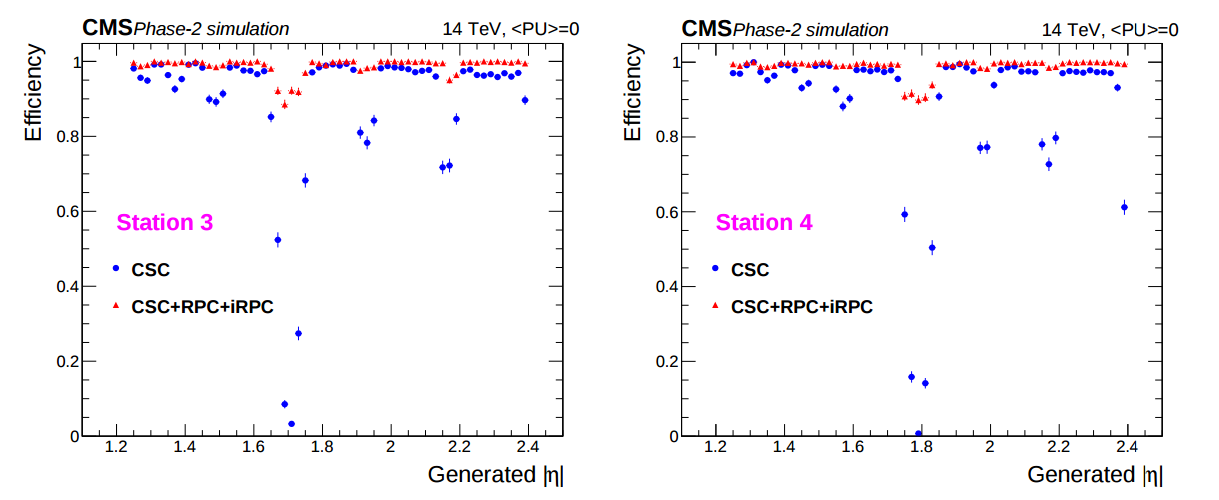
\includegraphics[width=\linewidth]{fig/chapt3/Trigger-efficiency-endcap.png}
		\caption{\label{fig:Endcap-trigger-eff} Simulation of the impact of RPC hit inclusion onto the local trigger primitive efficiency in station 3 (left) and station 4 (right). The contribution of iRPC starts above \psrape{1.8}.}
	\end{figure}
	
	Nevertheless, having only a single strip instead of pseudo-rapidity segmentation will increase the probability of double hits in the same channel. This probability was estimated to be low enough as it shouldn't exceed 0.7\%. This estimation was made assuming an average hit rate per unit area of \SI{600}{Hz/cm^2} in the iRPCs (see Figure~\ref{fig:iRPC-Rate}), a cluster size (average number of strips fired per muon) of 2, a strip active area of \SIsurface{158.4}{0.87}{cm} and a safety factor 3 leading to an estimated rate per strip of \SI{380}{kHz} corresponding to an average time interval of \SI{2600}{ns} in between 2 consecutive hits. The time for a signal to go through the full strip length is about \SI{10}{ns} to which can be added \SI{1}{ns} of dead time and 2 TDC clock cycles of \SI{2.5}{ns} for a minimal time interval of \SI{16}{ns} necessary to avoid ambiguities. The probability of having ambiguous double hits in a strip in then the ratio in between this minimal time interval in between 2 consecutive hits and the average time interval estimated from the rate the detectors are subjected to.
	
	The instantaneous luminosity at HL-LHC being very high, the rates at the level of the new chambers needed to be simulated in order to understand the necessary requirements for these detectors. The simulated results for different background components (neutrons, photons, electrons and positrons) are showed in Figure~\ref{fig:iRPC-Rate} assuming known sensitivities to these particles. It is showed that on average over the iRPC areas the rates would be of the order of \SI{600}{Hz/cm^2} (\SI{600}{Hz/cm^2} seen in RE3/1 and \SI{480}{Hz/cm^2} in RE4/1)~\cite{ANDREA2018}. Thus, taking into account a safety factor of about 3, it was decided that improved RPCs should at least be certified for rates reaching \SI{2}{kHz/cm^2} which would be achieved thanks to several improvements on the design and on the electronics. The detectors design will be based on the existing RPC design as they will be double gaps. Similarly to the existing RPC system, the electrode material will be HPL although the thickness of the electrodes and of the gas gap will be reduced to \SI{1.4}{mm} as a thinner gas gap leads to a decrease of deposited charge per avalanche as showed in Figure~\ref{fig:charge-gap}. The smaller the gas gap, the more the detector becomes sensitive to gap non-uniformities across the electrode planes making a gap of \SI{1.4}{mm} a good compromise in between these two competing factors.

	\begin{figure}[H]
		\centering
		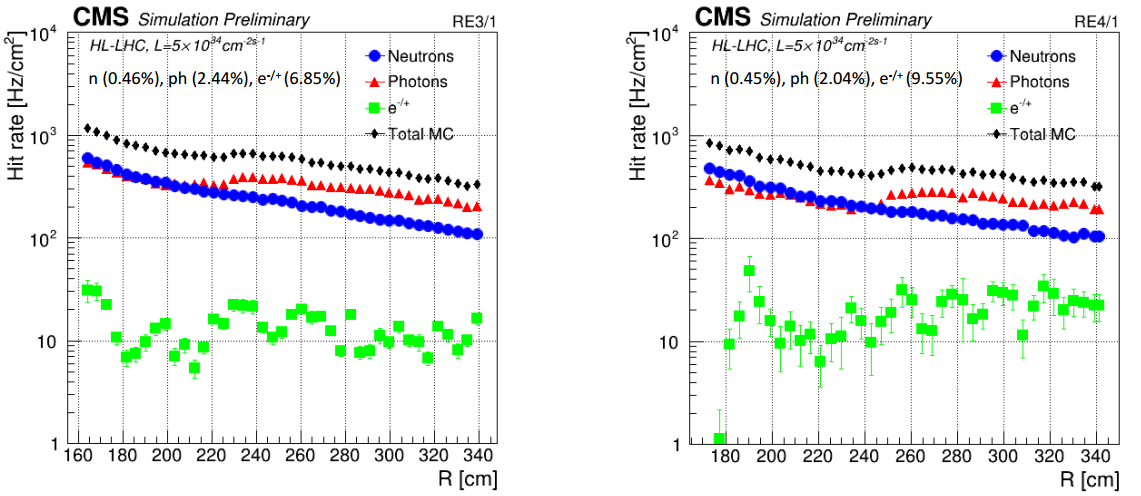
\includegraphics[width=\textwidth]{fig/chapt3/RPC-Sim-HL-LHC_Rate.png}
		\caption{\label{fig:iRPC-Rate} Expected hit rate due to neutrons, photons, electrons and positrons at HL-HLC instantaneous luminosity of $5\times10^{34}$ \si{cm^{-2}s^{-1}} in RE3/1 and RE4/1 chambers. The sensitivities of iRPCs used in the simulation for each particle are reported and differ from one endcap disk to another as the energies of the considered particles varies with the increasing distance from the interaction point.}
	\end{figure}

	\begin{figure}[H]
		\centering
		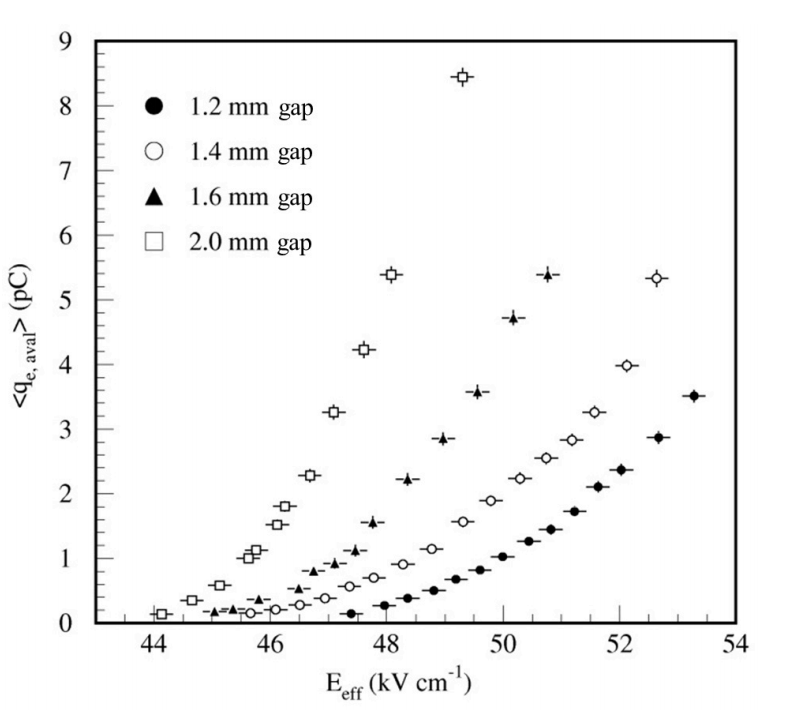
\includegraphics[width=0.8\plotwidth]{fig/chapt3/charge-vs-gap.png}
		\caption{\label{fig:charge-gap} Measured average charge per avalanche as a function of the effective electric field for different gas gap thickness in double gap RPCs using HPL electrodes.}
	\end{figure}
	
	A lower charge deposition inside of the detector volume means a slower ageing and a longer lifetime for detectors subjected to high irradiation. But, in order to take advantage of the lower detector gain, more sensitive electronics are required so that the part of gain that was formerly done in the gas volume can be moved to the electronics. Achieving this with the technology developed more than 10 years ago for the present system is not possible as the signal over noise ratio of such electronics doesn't allow to detect charges as low as \SI{10}{fC}. Moreover, the new front-end electronics will need to be radiation hard to survive to more than 10 years of HL-LHC conditions. The new technology that has been chosen is based on the PETIROC ASIC manufactured by OMEGA and is a 64-channel ASIC called CMS RPCROC. The properties of these electronics will be discussed in Chapter~\ref{chapt6}.
	
	\subsection{Installation schedule}
	\label{chapt3:ssec:schedule}
	
	The previous discussion on the different upgrade projects makes it clear that a lot of work is schedule for CMS to be ready at the end of LS3 for HL-LHC. Conducting all the upgrades of the muon system together with upgrades of the other subsystems like the replacement of the Tracker and of part of the ECAL, will prove to be very difficult as the opening of CMS to access the Barrel will be done by fully opening the endcaps leaving only the first disk to be accessible. Thus, most subsystems have planed early installation over LS2, and the following YETS until LS3 in order to give more space to LS3 schedule.
	
	First of all, LS2 will see the installation of GE1/1 detectors, all the on-detector schedule of CSCs and the installation of the necessary services for the improved RPCs to be installed later, such as the HV and LV power supply lines, the gas and cooling lines or signal cables. CSCs will have a huge work to do during LS2 as they will need to extract all of their detectors to refurbish them with upgraded DCFEB and ALCT mezzanine boards. The GE1/1 services were installed during LS1 together with a few demonstrator and only the detectors needs to be integrated into the first endcap disk. The detectors are presently being built and tested at the different assembly site to prepare for a smooth LS2 work.
	
	The work of GEMs will be continued during the following YETS during which is planned the installation of the GE2/1 stations to only leave the ME0 to be installed during LS3. The iRPC program will follow a similar path as the new detectors will be installed during the YETS preceding LS3 in prevision of the fact that the endcap disks will not be accessible during LS3. This way, all the subsystems, but DTs, made great effort on planing their installation and integration within CMS only to have to deal with off-detector issues during the LS3 period, such as the replacement of ODMBs and HV system in the case of CSCs or the upgrade of the RPC Link System. Finallly, during LS3 are schedules the replacement of DT minicrates electronics and the installation and integration of ME0 GEMs together with the HGCAL.
	
\section{Implications of the different upgrades on the Level-1 Trigger. Improvement of physics performance.}
\label{chapt3:sec:L1tP2}

	The upgrades of the different subsystems will have a subsequent impact on the Level-1 Trigger. Indeed, although its main scheme will not be affected, the efficiency of the trigger in efficiency identifying muons and provide the DAQ with good and fast trigger that can cope with HL-LHC instantaneous luminosity is a major improvement. In addition to the upgrade of the muon system in terms of trigger accept rate and latency, the Level-1 Trigger will get extra information in including the Tracker Trigger into its Muon Track Finder logic and combine the L1 Muon Trigger with Tracker and Calorimeter Triggers to generate a Global L1 Trigger with a much better momentum resolution, as showed in Figure~\ref{fig:L1-trigger}.

	\begin{figure}[H]
		\centering
		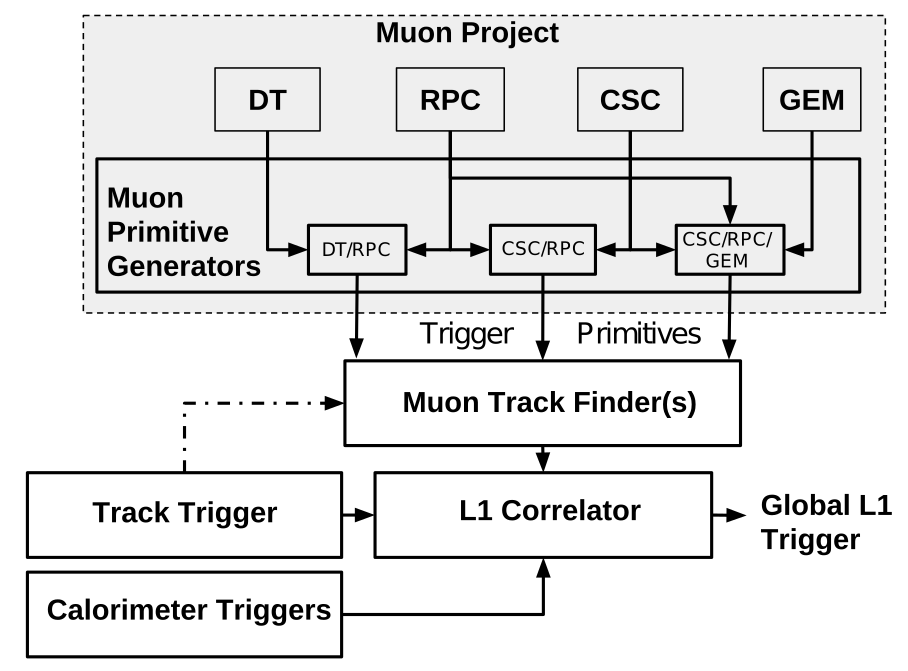
\includegraphics[width=\plotwidth]{fig/chapt3/Phase-II-L1-Trigger.png}
		\caption{\label{fig:L1-trigger} Data flow of the Level-1 Trigger during Phase-II operations.}
	\end{figure}
	
	In terms of muon trigger, 3 regions are considered due to their different track finding logic: the \acf{BMTF}, the \acf{EMTF} for both the barrel and endcap regions, and finally the \acf{OMTF} which concerns the pseudo-rapidity region in which there is a common coverage by both the barrel and endcap muon systems. This region can be seen in Figure~\ref{fig:P2Quadrant} for \psrapr{0.9}{1.2} and requires a specific more complex logic to provide with an efficient reconstruction of the muons due to the different orientation of the detectors and of the more complex magnetic field of this region that needs to be taken into account. The benefits of the upgrade for each of these track finders will be coming from different improvements and will be detailed sector by sector.
	
	The main contribution to the improvement of the BMTF is the time resolution improvement of RPC link systems that will allow to take profit of the full \SI{1.5}{ns} resolution of the detectors. From the perspective of RPCs only, this improvement will help reducing the neutron induced background and slightly improve the bunch crossing assignment. The upgrade of DT electronics is also to take into account as the trigger primitive generator will be renewed through the use of TDCs that will send the digitized signals directly to the back-end electronics instead of having an on-detector trigger logic as it will be the case until the end of Phase-I. The front data of both DTs and RPCs will be sent to the same back-end electronics. These upgrades were detailed in section~\ref{chapt3:sec:electronics} and will lead to a more robust operation of the trigger in the barrel region. Indeed, the combination of RPC hits together with DT primitives will bring improvement in the bunch crossing assignment and improve the efficiency of the trigger in between the wheels were the quality of DT primitives is the poorest. Moreover, having a redundant information is important in the case of failure and loss of efficiency of one of either subsystems.
	
	\begin{figure}[H]
		\begin{subfigure}{0.5\linewidth}
			\centering
			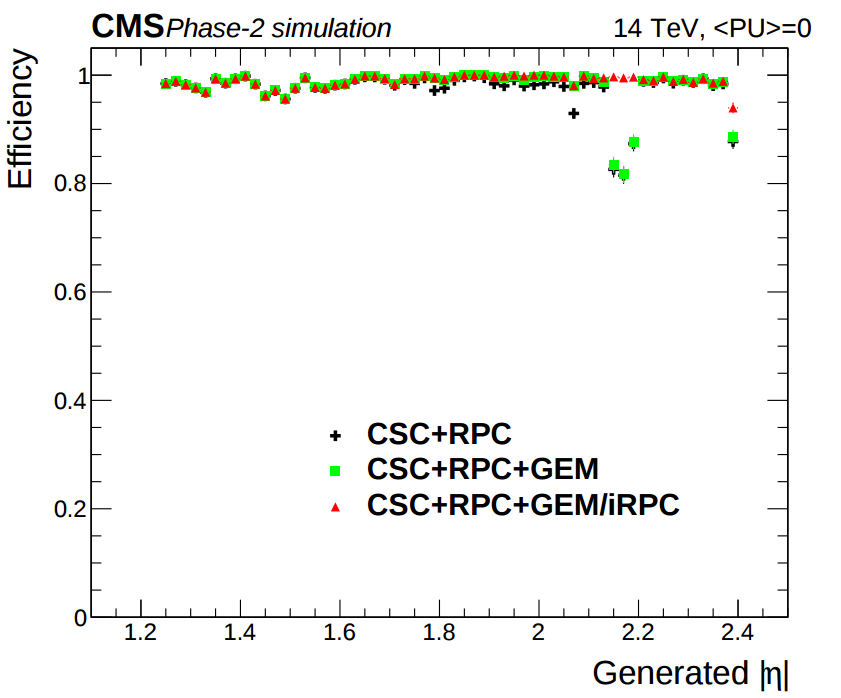
\includegraphics[height=5cm]{fig/chapt3/EMTF-eff-2of4.png}
			\caption{\label{fig:EMTF-eff:A}}
		\end{subfigure}
		\begin{subfigure}{0.5\linewidth}
			\centering
			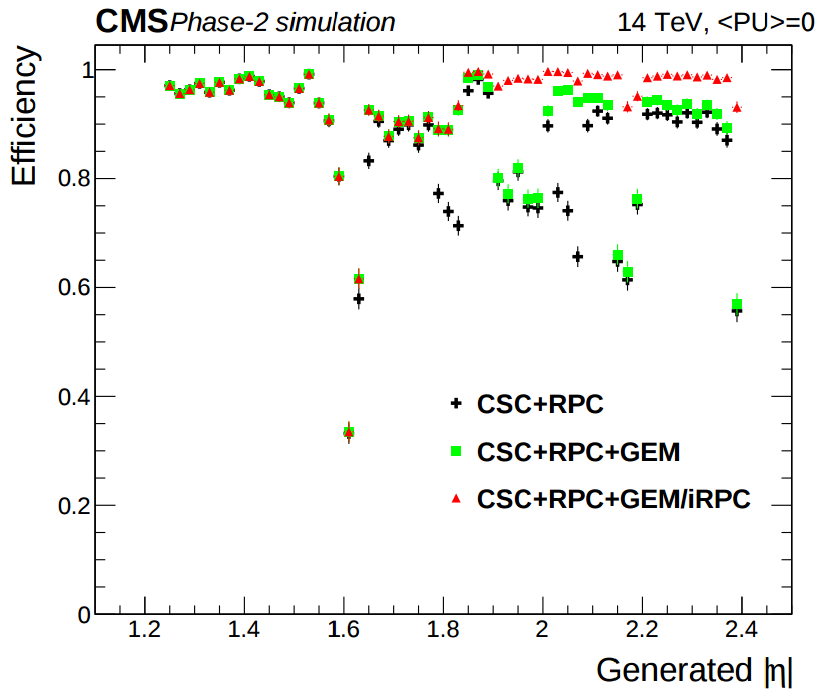
\includegraphics[height=5cm]{fig/chapt3/EMTF-eff-4of4.png}
			\caption{\label{fig:EMTF-eff:B}}
		\end{subfigure}
		\caption{\label{fig:EMTF-eff} Efficiency of the L1 trigger in the endcap region after Phase-II upgrade in the case CSC/GEM/RPC hits are requested in at least 2 stations out of four (\ref{fig:EMTF-eff:A}) and in all four stations (\ref{fig:EMTF-eff:B}).}
	\end{figure}

	\begin{figure}[H]
		\centering
		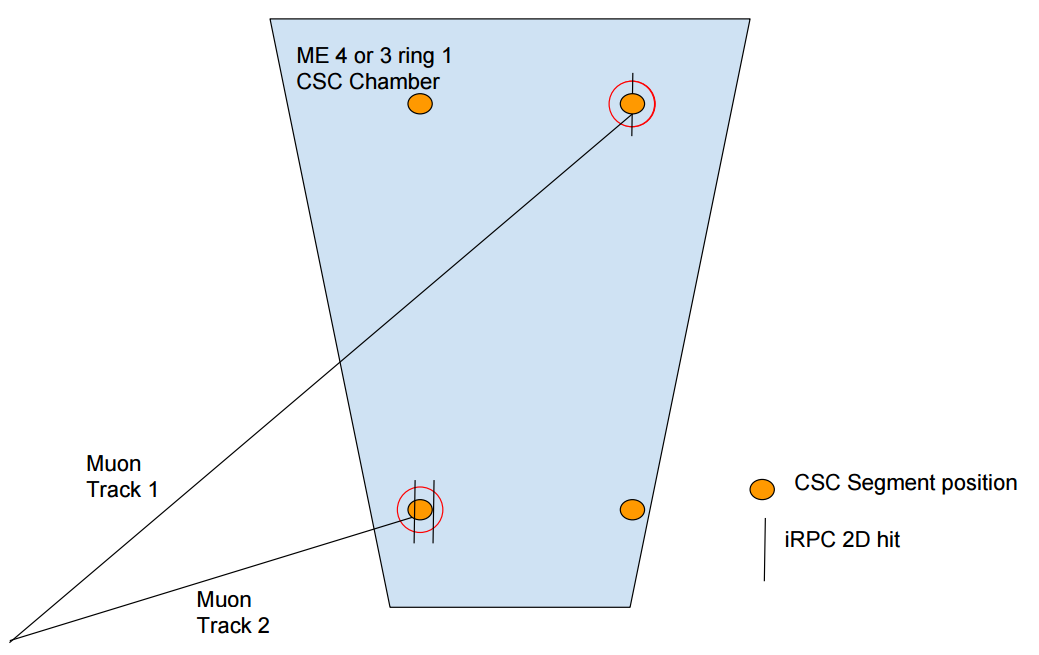
\includegraphics[width=0.9\plotwidth]{fig/chapt3/CSC-LCT-ambiguity.png}
		\caption{\label{fig:LCT-ambiguity} Resolution of the LCT ambiguous events thanks to the combination of CSC and iRPC readout data. Using CSCs only, 2 pairs of hits are possible.}
	\end{figure}
	
	With new detectors to cover the very forward region and the upgrade of RPC Link System, the EMTF will be greatly improved. The current EMTF already use more sophisticated algorithms by combining together RPC hits and CSC primitives and will also benefit from the improved time resolution of the RPC system. The GEMs, in stations 1 and 2, and the iRPCs, in stations 3 and 4, will be added into the EMTF algorithm. Both these contributions will help increasing the efficiency of the L1 trigger in the endcap region in one hand, as showed by Figure~\ref{fig:EMTF-eff}, and help lowering the L1 trigger rate in the other hand, especially in the most forward region. The improvement of the efficiency will come both from the better time resolution of RPC link boards and from the addition of more hits along the muon tracks and also a contribution from the GEMs to the lever arm of each track thanks to there high angular resolution.
	
	The rate will be partly reduced in the forward region thanks to the better spatial resolution of iRPCs, with respect to the current RPC system, that will reduce the ambiguity brought by multiple local charged tracks in CSCs, as explained through Figure~\ref{fig:LCT-ambiguity}. Indeed, as the rates will increase, the probability to record more than a single local charged track will greatly increase. This is due to the fact that the trigger algorithm uses information from 3 consecutive bunch crossings to find muon tracks. It is estimated that with iRPCs operated at 95\% efficiency the resolution of ambiguous events would be of the order of 99.7\%.
	
	\begin{figure}[H]
		\begin{subfigure}{0.5\linewidth}
			\centering
			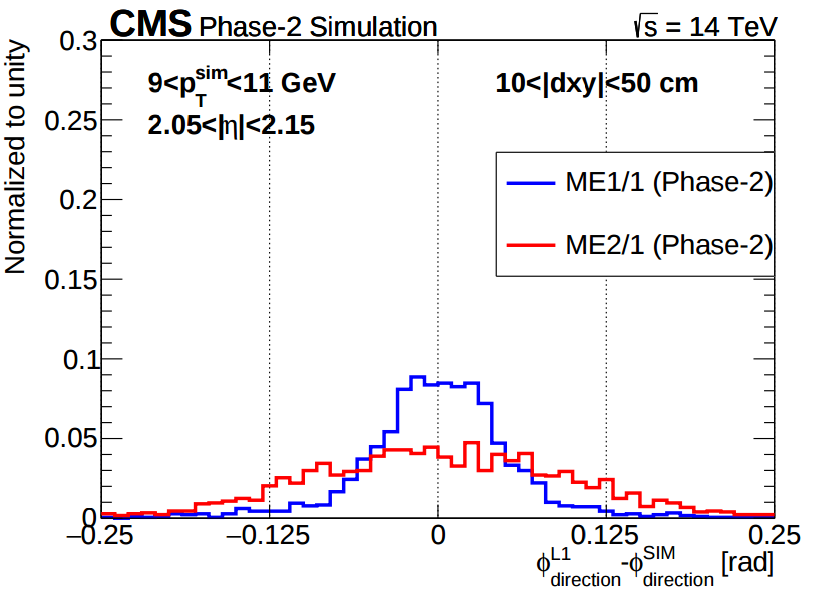
\includegraphics[height=5cm]{fig/chapt3/CSC-angular-res.png}
			\caption{\label{fig:CSC-GEM-res:A}}
		\end{subfigure}
		\begin{subfigure}{0.5\linewidth}
			\centering
			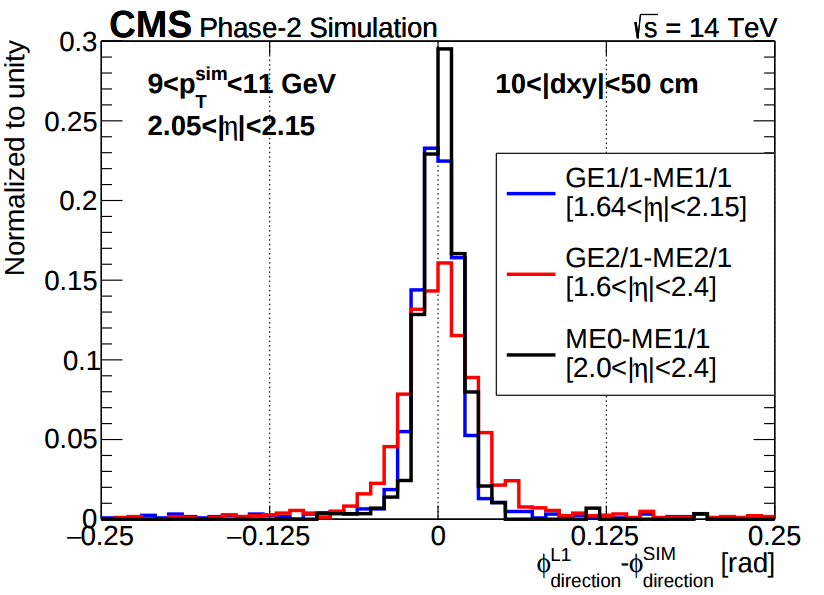
\includegraphics[height=5cm]{fig/chapt3/GEM-angular-res.png}
			\caption{\label{fig:CSC-GEM-res:B}}
		\end{subfigure}
		\caption{\label{fig:CSC-GEM-res} The angular resolution on reconstructed muon tracks in the GEM overlap region \psrapr{2.0}{2.15} is compared for Phase-II conditions in the case CSC are alone (Figure~\ref{fig:CSC-GEM-res:A}) and in the case the GEMs' data, including ME0, is combined to which of CSCs (Figure~\ref{fig:CSC-GEM-res:B}).}
	\end{figure}
	
	\begin{figure}[H]
		\begin{subfigure}{0.5\linewidth}
			\centering
			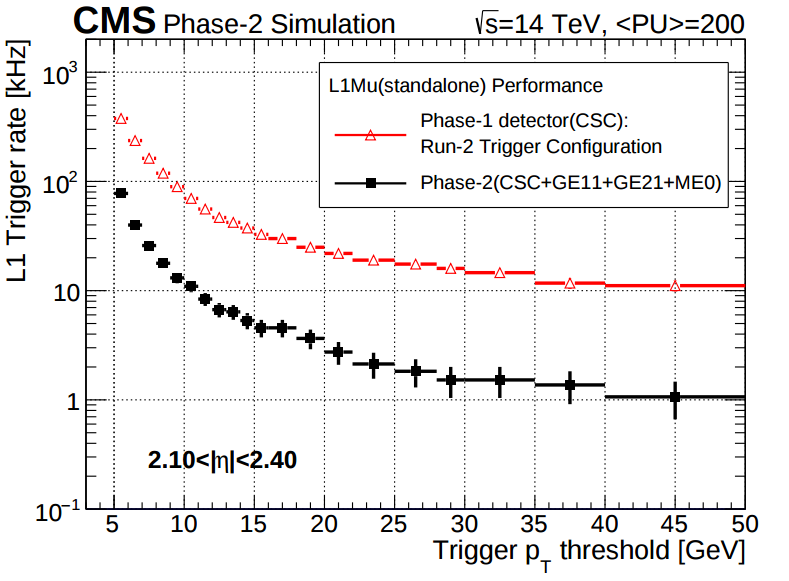
\includegraphics[height=5cm]{fig/chapt3/GEM-trigger-rate.png}
			\caption{\label{fig:CSC-GEM-perf:A}}
		\end{subfigure}
		\begin{subfigure}{0.5\linewidth}
			\centering
			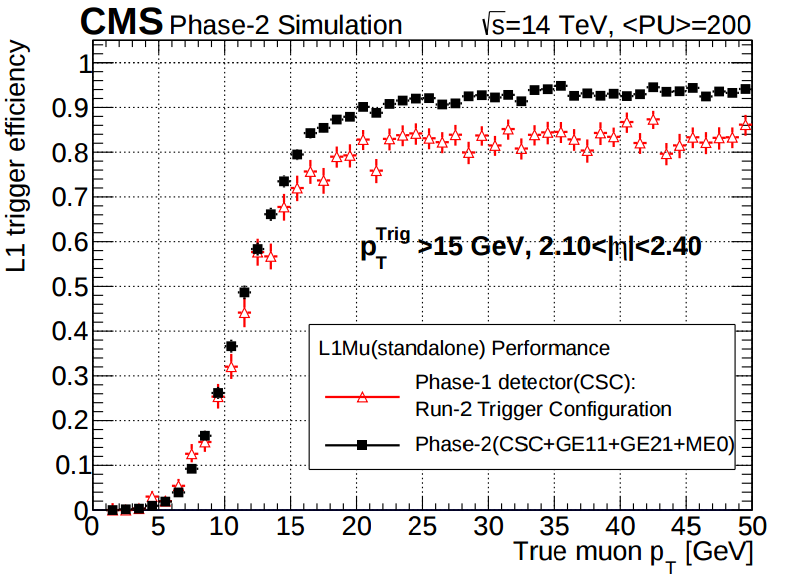
\includegraphics[height=5cm]{fig/chapt3/GEM-trigger-eff.png}
			\caption{\label{fig:CSC-GEM-perf:B}}
		\end{subfigure}
		\caption{\label{fig:CSC-GEM-perf} Comparison of L1 trigger performances for prompt muons with and without the addition of GEMs in the region \psrapr{2.1}{2.4} at Phase-II conditions. GEMs would allow a reduction of the trigger accept rate by an order of magnitude (Figure~\ref{fig:CSC-GEM-perf:A}) while increasing the trigger efficiency (Figure~\ref{fig:CSC-GEM-perf:B}).}
	\end{figure}
	
	The addition of GEMs will improve greatly the measured muon momentum resolution by improving the global resolution of the direction of muon tracks, as can be seen in Figure~\ref{fig:CSC-GEM-res}, which will contribute to lowering the trigger rate and increase the efficiency, as can be seen from Figure~\ref{fig:CSC-GEM-perf} that focuses especially in the most challenging pseudo-rapidity region. Data from both CSCs and GEMs are combined into the OTMB to build on each station, GEM/CSC primitives matching space and time information from both subsystems.
	
	Finally, the development of a track finder specific to the overlap region was already achieved during the Phase-I upgrade of the L1-Trigger~\cite{L1UPGRADE2016}. Nevertheless, the improvements of DT spatial resolution and RPC timing will be carried and implemented into the OMTF.

\section{Ecofriendly gas studies}
\label{chapt3:sec:EcoGas}

	Future strict restrictions in the use of certain gases will affect the gaseous detectors of several experiment, including CMS. The European Commission adopted a new "F-gas regulation" in 2014~\cite{EUFGAS2014} with the goal to strongly control and reduce the use of fluorinated gases with high \acf{GWP}. Using $CF_4$, $C_2H_2F_4$ and $SF_6$, both CSC and RPC subsystems will need to address this problem by finding new gas mixture for the operation of their detectors. Finding a replacement for these gas component that were used for very specific reasons will be a great challenge. Indeed, CSCs use $CF_4$ in order to enhance the longevity of the detectors, increase the drift velocity of electrons and quench photons with a non-flammable gas mixture. RPCs use a mixture mainly composed of $C_2H_2F_4$, or \textit{R134a}, that features a high effective Townsend coefficient and the great average fast charge allowing for operations with a high threshold, and contains a small fraction of $SF_6$ that is used for its electronegative properties that prevents the development of delta-rays in the gas volume that might trigger multiple ionization and avalanches.
	
	\begin{table}[H]
		\centering
		\begin{tabular}{l c c}
			\hline
			 & CSC & RPC\\
			\hline
			Greenhouse gases used & $CF_4$ & $C_2H_2F_4$ and $SF_6$ \\
			Greenhouse gases fraction in the gas mixture & 10\% & 95.2\% and 0.3\% \\
			Global Warming Potential (relative to $CO_2$) & 6500 & 1300 and 23900 \\
			Gas mixture re-circulation & Yes, 90\% & Yes, 85\% \\
			Gas mixture replenishing rate (\si{l/hr}) & 700 & 1100 \\
			F-gas recuperation & Yes, $\approx$40\% & No \\
			F-gas venting rate (\si{l/hr}) & 42 & 1047 and 3.3 \\
			$CO_2$-equivalent rate (\si{m^3/h}) & 273 & 1440 \\
			Relative impact (entire muon system = 100\%) & 16\% & 84\% \\
			\hline
		\end{tabular}
		\caption{\label{tab:F-GAS-CMS} Details of the greenhouse fluorinated gases used in CMS and of their GWP~\cite{PHASEIITP}.}
	\end{table}
	
	Nevertheless, all these gases have a very high GWP, as reported in Table~\ref{tab:F-GAS-CMS}, and only few options are left. The subsystems need to work on strongly decrease the loss of these gases due to leaks in the gas system or completely change their gas mixture for more ecofriendly ones. Reducing the amount of F-gas released in the atmosphere due to leaks on the current gas system will require installation of a F-gas recuperation system on RPCs side and an upgrade of CSCs existing one in addition to the repair of existing leaks. With such measures, it is expected that the total rate of greenhouses gas vented in the atmosphere would represent only 1.6\% of the current levels~\cite{PHASEIITP}. In the most critical case the F-gas were to be banned, it would be necessary to have replacement mixtures to operate CMS. CSC is presently investigating replacement for $CF_4$ such as $CF_3I$, $C_4F_6$, $IC_3F_6$, $C_3F_8$ or $CHF_3$ while RPCs, in collaboration with the ATLAS RPC group which uses the same gas mixture and, hence, faces similar restrictions, have identified $CF_3I$ (GWP $\leq$ 1) and $C_3H_2F_4$ (GWP < 1), referred to as HFO-1234ze, as potential candidates with mixtures containing $CO_2$ but more R\&D needs to be conducted for both subsystems before concluding on the best alternative. No good alternative to the present mixtures will require very efficient abatement system in CMS to burn and convert the greenhouse gases into less harmful ones. This way, the air pollution would be strongly reduced.
	
	\begin{figure}[H]
		\hspace*{-0.1\linewidth}
		\begin{subfigure}{0.6\linewidth}
			\centering
			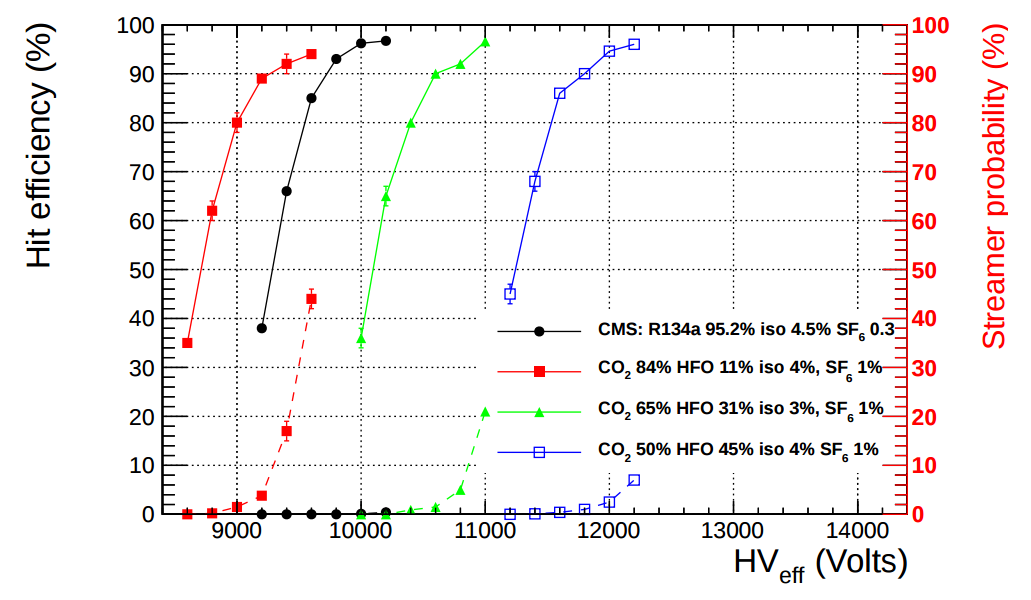
\includegraphics[height=5cm]{fig/chapt3/HFO-mixtures.png}
			\caption{\label{fig:RPC-eco:A}}
		\end{subfigure}
		\begin{subfigure}{0.6\linewidth}
			\centering
			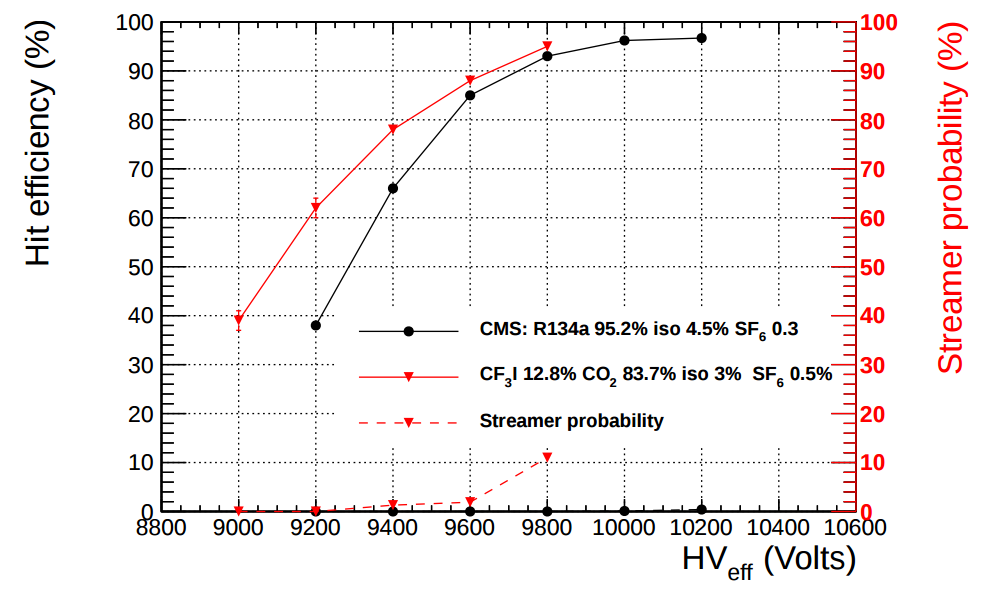
\includegraphics[height=5cm]{fig/chapt3/CF3I-mixture.png}
			\caption{\label{fig:RPC-eco:B}}
		\end{subfigure}
		\caption{\label{fig:RPC-eco} The efficiency (solid lines) and streamer probability (dashed lines) of $HFO$/$CO_2$ (Figure~\ref{fig:RPC-eco:A}) and $CF_3I$/$CO_2$ (Figure~\ref{fig:RPC-eco:B}) based gas mixtures as a function of the effective high-voltage are compared with the present CMS RPC gas mixture represented in black. The detector used for the study is a single gap RPC with similar properties than CMS RPCs. The streamer probability is defined as the proportion of events with a deposited charge greater than \SI{20}{pC}.}
	\end{figure}
	
	The status of RPC studies are presented in Figure~\ref{fig:RPC-eco} in which the performance (efficiency and streamer probability) of an RPC operated with alternative gas mixtures is compared to the present CMS RPC mixture. Although the efficiency of detectors operated with mixtures containing $CO_2$/$CF_3I$ or $CO_2$/$HFO$ as a replacement for $C_2H_2F_4$ seem to reach similar levels than which of the detectors operated with the present mixture, the new gas mixtures feature a streamer probability (probability to have very large avalanches whose induced charge is greater than \SI{20}{pC}) that far exceeds which of the present fluorinated mixture. The $SF_6$, being a component of the mixture added in order to reduce the probability of large avalanches thanks to its electronegativity, doesn't seem to prevent streamers as efficiently even when used at levels more than 3 times higher than with the standard CMS RPC mixture. Nevertheless, it is important to note that these results were obtained with a single gap RPC while the use of a double gap RPC would reduce the operation voltage by 200 to \SI{300}{V}, lowering the induced charge. A compromise in between good efficiency and acceptable level of streamer probability and the fine tuned composition of potential replacement gas mixtures will be studied using a standard double-gap CMS RPC.

\clearpage{\pagestyle{empty}\cleardoublepage}